\section{Figures}
\label{figures}
%%% Please be aware that for original research articles we only permit a combined number of 15 figures and tables, one figure with multiple subfigures will count as only one figure.
%%% Use this if adding the figures directly in the mansucript, if so, please remember to also upload the files when submitting your article
%%% There is no need for adding the file termination, as long as you indicate where the file is saved. In the examples below the files (logo1.eps and logos.eps) are in the Frontiers LaTeX folder
%%% If using *.tif files convert them to .jpg or .png
%%%  NB logo1.eps is required in the path in order to correctly compile front page header %%%
% \begin{center}



% Section 2
\begin{figure}
    \centering
    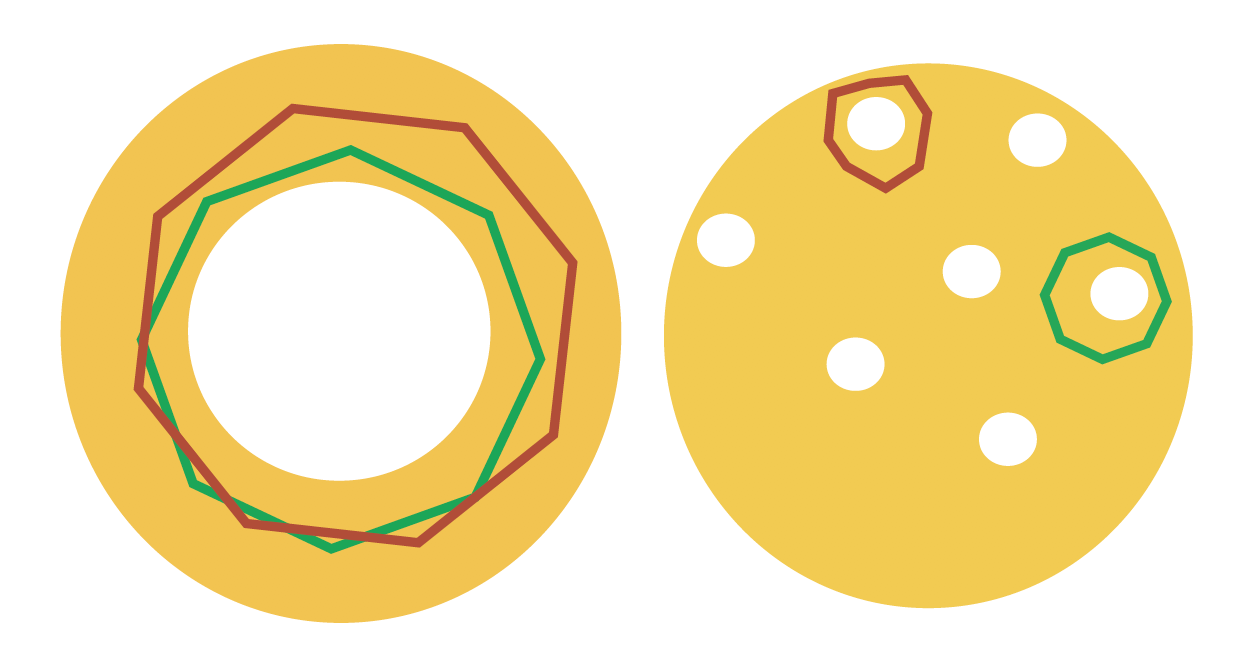
\includegraphics[width=0.8\textwidth]{figures/generatorExample.png}
    \caption{Two disks (yellow) --- which we regard as 2-dimensional simplicial complexes, though the explicit decomposition into simplices is not shown --- with different numbers of holes (white) and cycle representatives (red or green) from \cite{Carlsson2009TopologyAD}. The disk on the left has a single 2-dimensional  ``hole'' ($\beta_1 = 1$), and the two loops around it are cycle representatives for the same homology class. Similarly, the disk on the right has seven ``holes'' ($\beta_1 = 7$) and the two loops shown are cycle representatives for different homology classes.
    }
    \label{fig:generatorExamples}
\end{figure}


\begin{figure}[h!]
\begin{center}
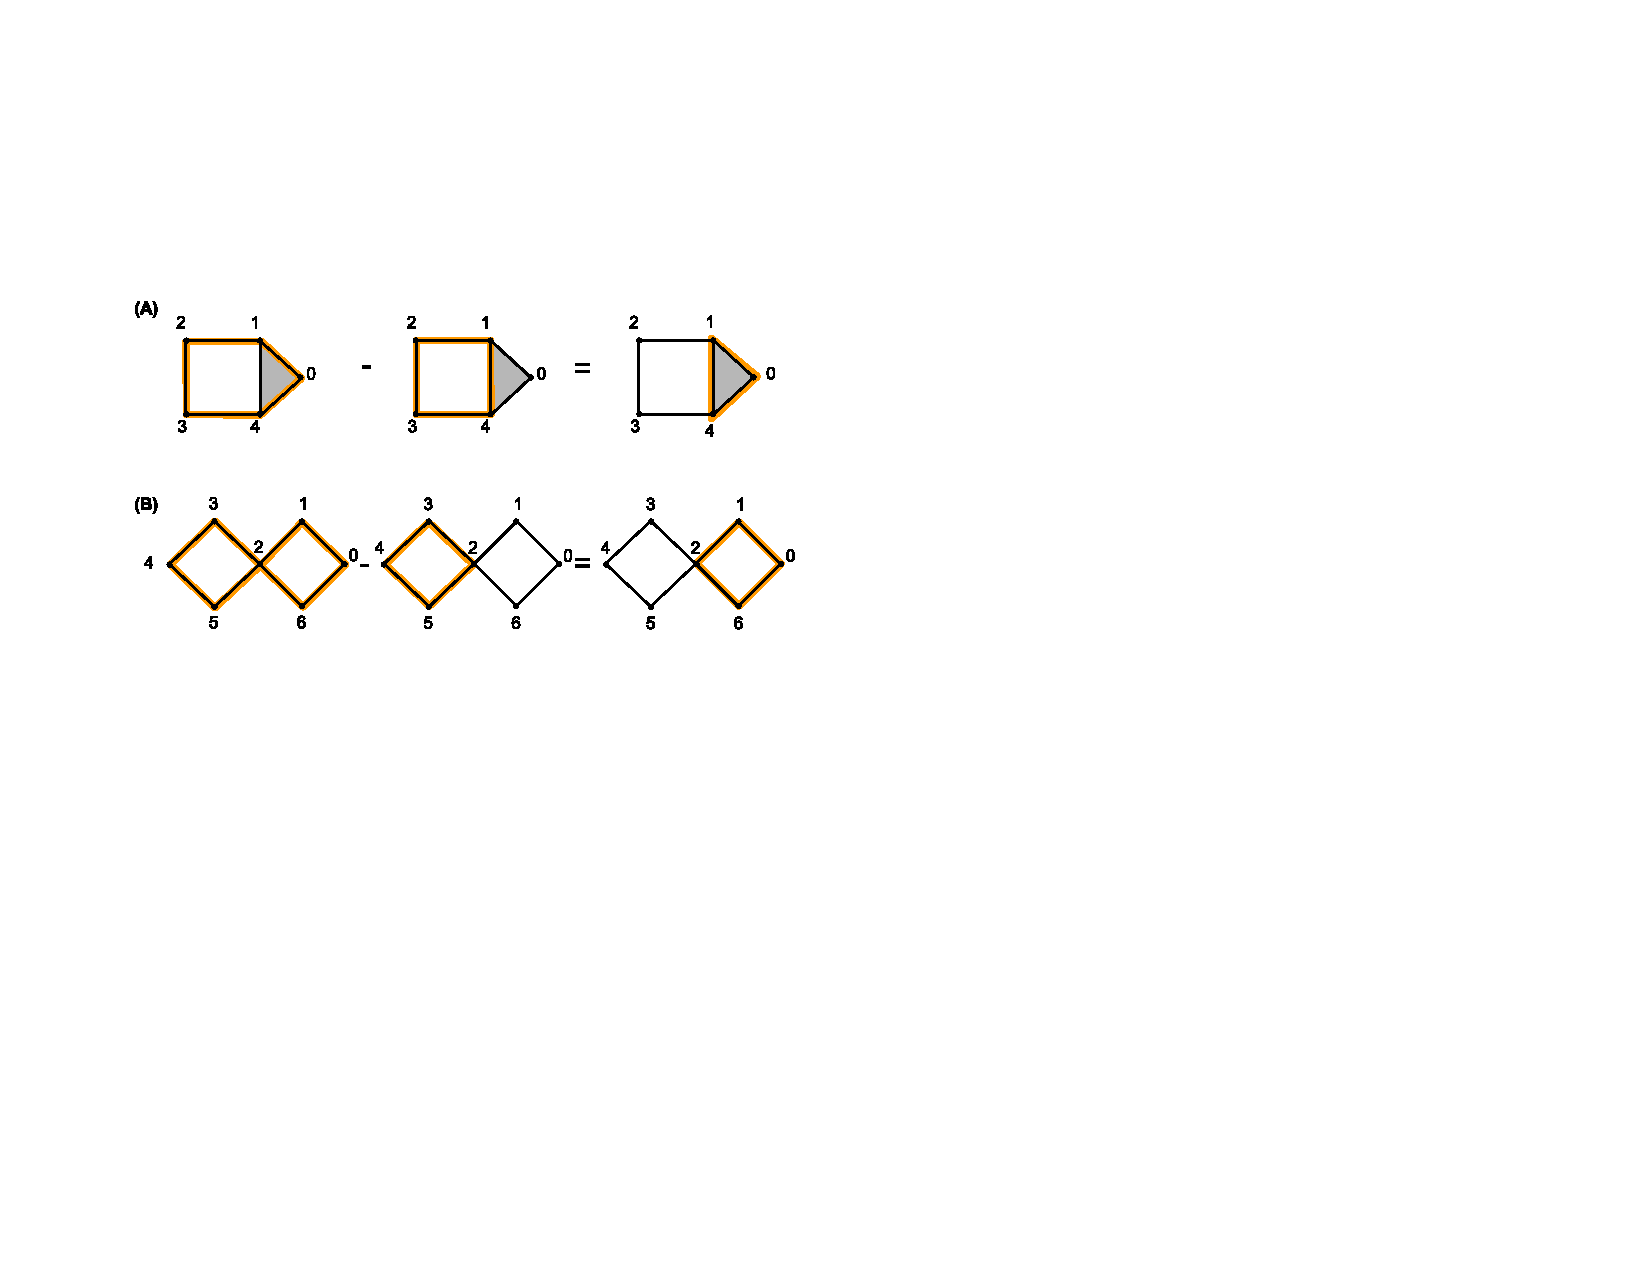
\includegraphics[width=1\textwidth]{figures/examplesorange.pdf}% This is a *.eps file
\end{center}
\caption{We show an example of homologous cycles in \textbf{(A)}, taken from \cite{TZH15}. The 1-cycle $(0,1) + (1,2) + (2,3) + (3,4) - (0,4)$ and the 1-cycle $(1,2) + (2,3) + (3,4) - (4,1)$ are homologous because their difference is the boundary of $(0,1,4)$. Subfigure \textbf{(B)} shows an example of non-homologous cycles. The 1-cycle $(\sum_{i=0}^4 (i, i+1))-(5,2)+(2,6)-(0,6)$ and the 1-cycle $(2,3) + (3,4)+(4,5)-(2,5)$ are not homologous because their difference is a cycle $(0,1)+(1,2)+(2,6)-(0,6)$ which is not a linear combination of boundaries of 2-simplices. } \label{fig:boundaryexample}
\end{figure}
% Section 3
\begin{figure}[h!]
\begin{center}
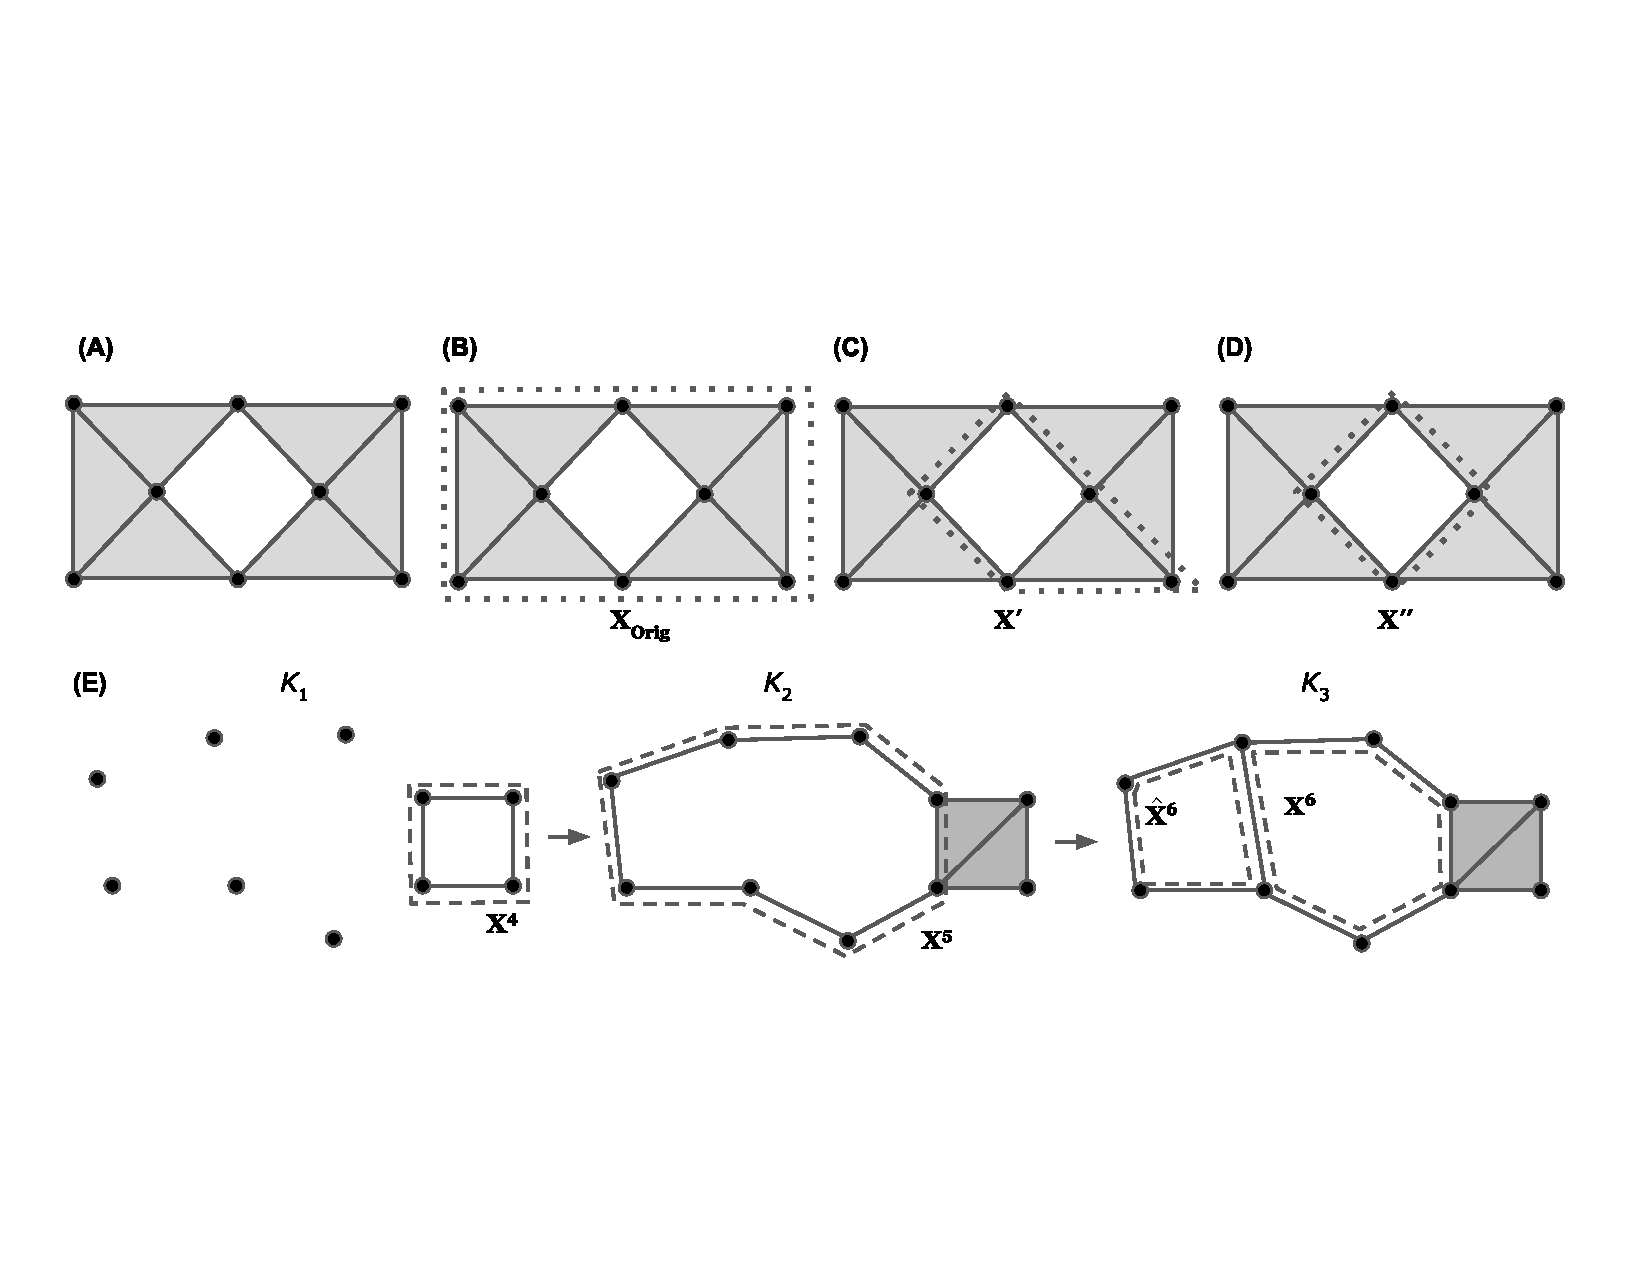
\includegraphics[width=1\textwidth]{figures/examplesminimal.pdf}% This is a *.eps file
\end{center}
\caption{Examples of optimizing a cycle representative (using the notion of minimizing edges) within the same homology class (\textbf{A-D}) and using a basis of cycle representatives (\textbf{E}), modified examples taken from \cite{Escolar2016} and \cite{Obayashi2018}. The dotted lines represent a cycle representative for the enclosed ``hole''. Intuitively, we consider $\optimalrep''$ in (\textbf{D}) as the optimal cycle representative since it consists of the smallest number of edges. Subfigure (\textbf{E}) shows a case where we optimize a cycle representative using a basis of cycle representatives. In (\textbf{E}), $\{\optimalrep^4, \optimalrep^5, \optimalrep^6\}$ is the original basis of cycle representatives. We can substitute $\optimalrep^6$ with $\hat{\optimalrep}^6$, which we can obtain by adding $\optimalrep^5$ to $\optimalrep^6$, and thus obtain $\{\optimalrep^4, \optimalrep^5, \hat{\optimalrep}^6\}$ as the new basis of cycle representatives.}\label{fig:example-optimal}
\end{figure}

\begin{figure}[h!]
\begin{center}
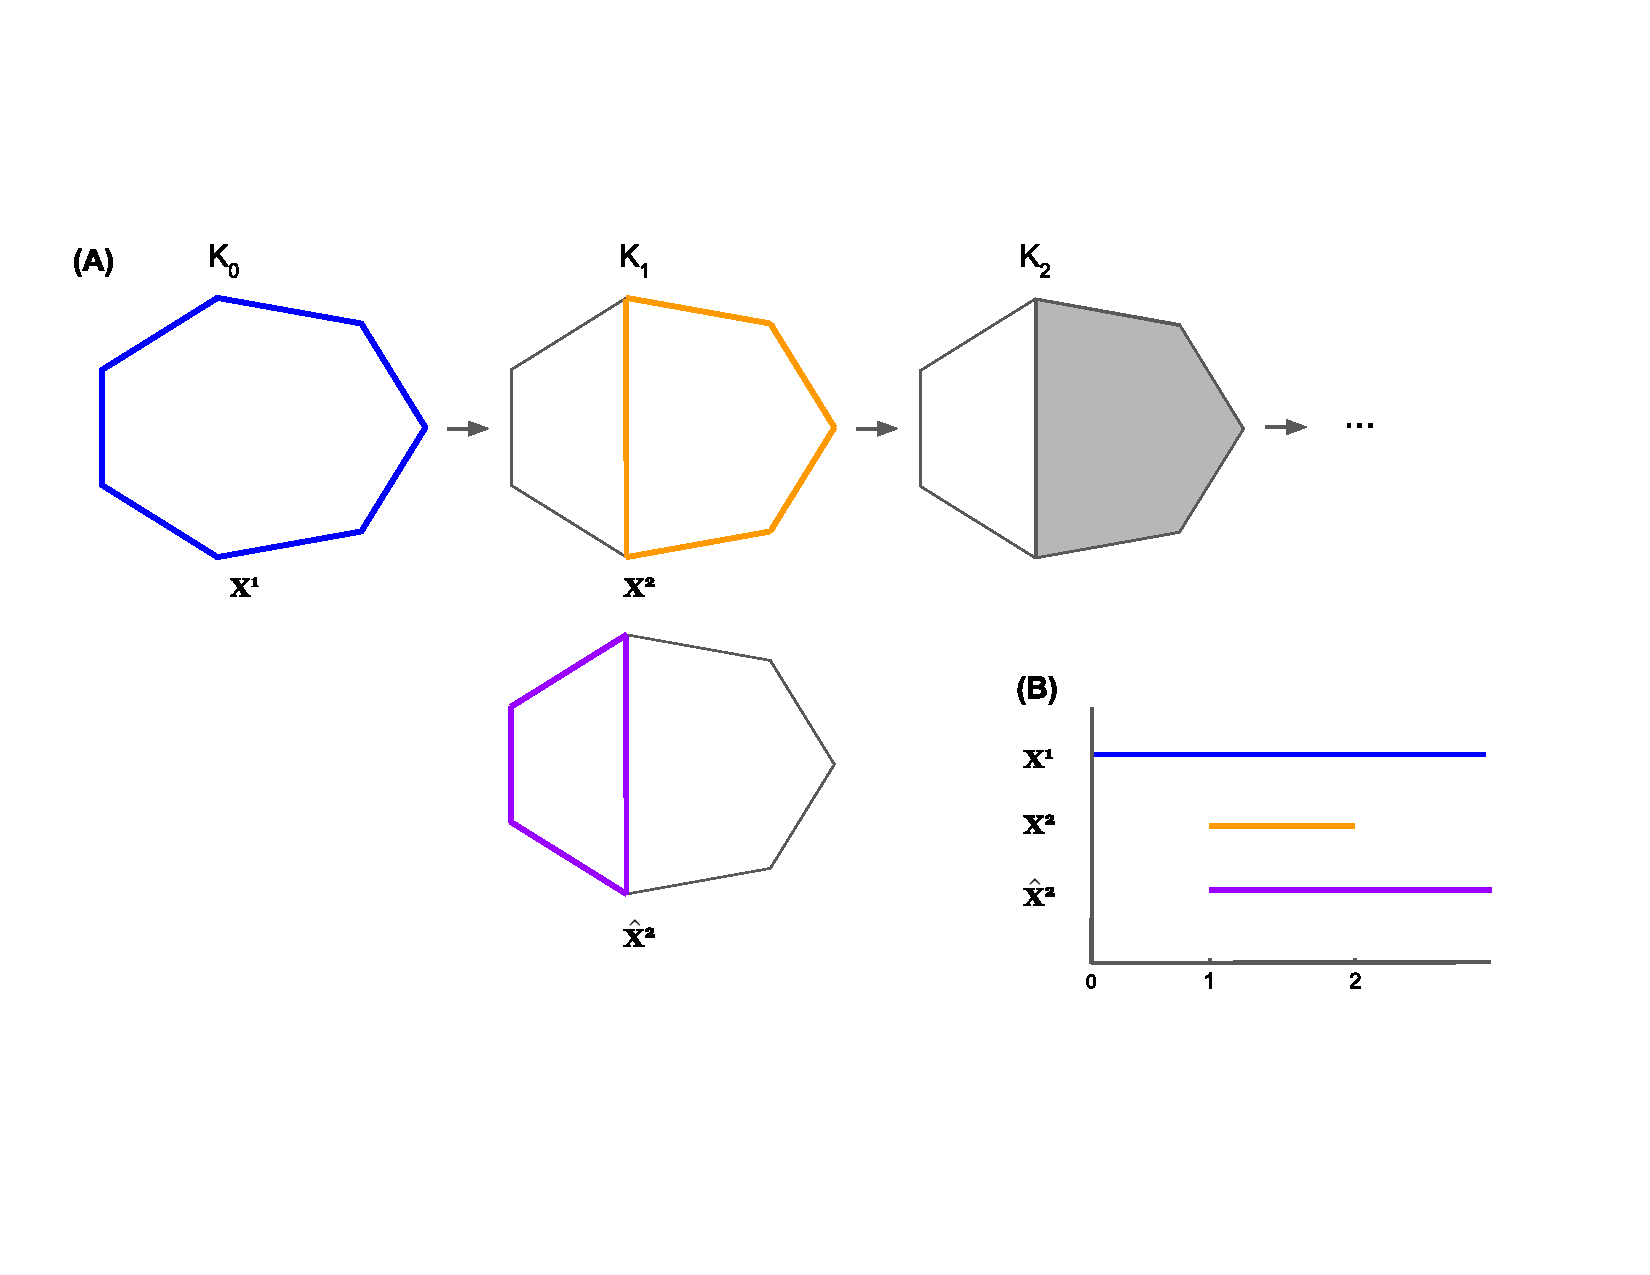
\includegraphics[width=1\textwidth]{figures/gregExample.pdf}% This is a *.eps file
\end{center}
\caption{An example where the optimal cycles obtained from \pr \eqref{eq:escolarargmin} do not form a persistent homological cycle basis. The thickened colored cycles in Subfigure (\textbf{A}) represent a cycle representative for the hole it encloses, and the bar with the corresponding color in Subfigure (\textbf{B}) records the lifespan of the cycle. In Subfigure (\textbf{A}), we see $\persinterval(\optimalrep^1) = [0,\infty), \persinterval(\optimalrep^2) = [1,2).$ Then, $\{\optimalrep^1, \optimalrep^2\}$ forms a basis for the persistent homological cycles. The cycle representative $\hat \optimalrep^2$ is an optimal cycle representative obtained by solving \pr (\ref{eq:filteredminimalbasis}) for the filtered simplicial complex $K_2$. However, $\persinterval(\hat \optimalrep_2) = [1, \infty)$, and thus  $\{\optimalrep^1, \hat \optimalrep^2\}$ is no longer a persistent homological cycle basis.} \label{fig:example-persBasis}
\end{figure}

\begin{figure}[h!]
\begin{center}
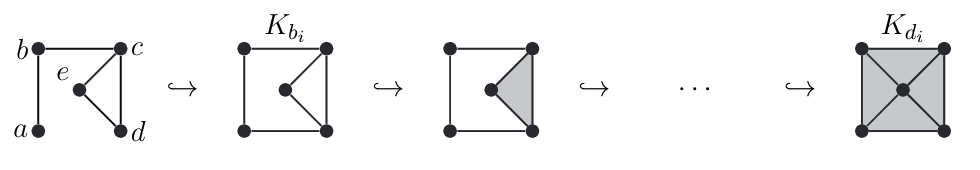
\includegraphics[width=1\textwidth]{figures/volumeexample.jpg}% This is a *.eps file
\end{center}
\caption{A situation in which a volume-optimal cycle is different from the uniform minimal cycle. Consider the filtered simplicial complex pictured. For the persistence interval $[b_i,d_i)$, the cycle with minimal $0$-norm (fewest number of edges) is $(a,b) + (b,c) + (c,d)  + (d,a)$.
However, the volume-optimal cycle would be found as follows: considering $K_{d_i}$, we must find the fewest $2$-simplices whose boundary captures the persistence interval. In this case, we would have an optimal volume $(a,b,e) + (b,c,e) + (a,d,e)$ and volume-optimal cycle $(a,b) + (b,c) + (c,e) + (e,d) + (d,a)$. 
}\label{fig:volumeoptimal}
\end{figure}
% section 4
%
 \begin{figure}[h!]
 \begin{center}
 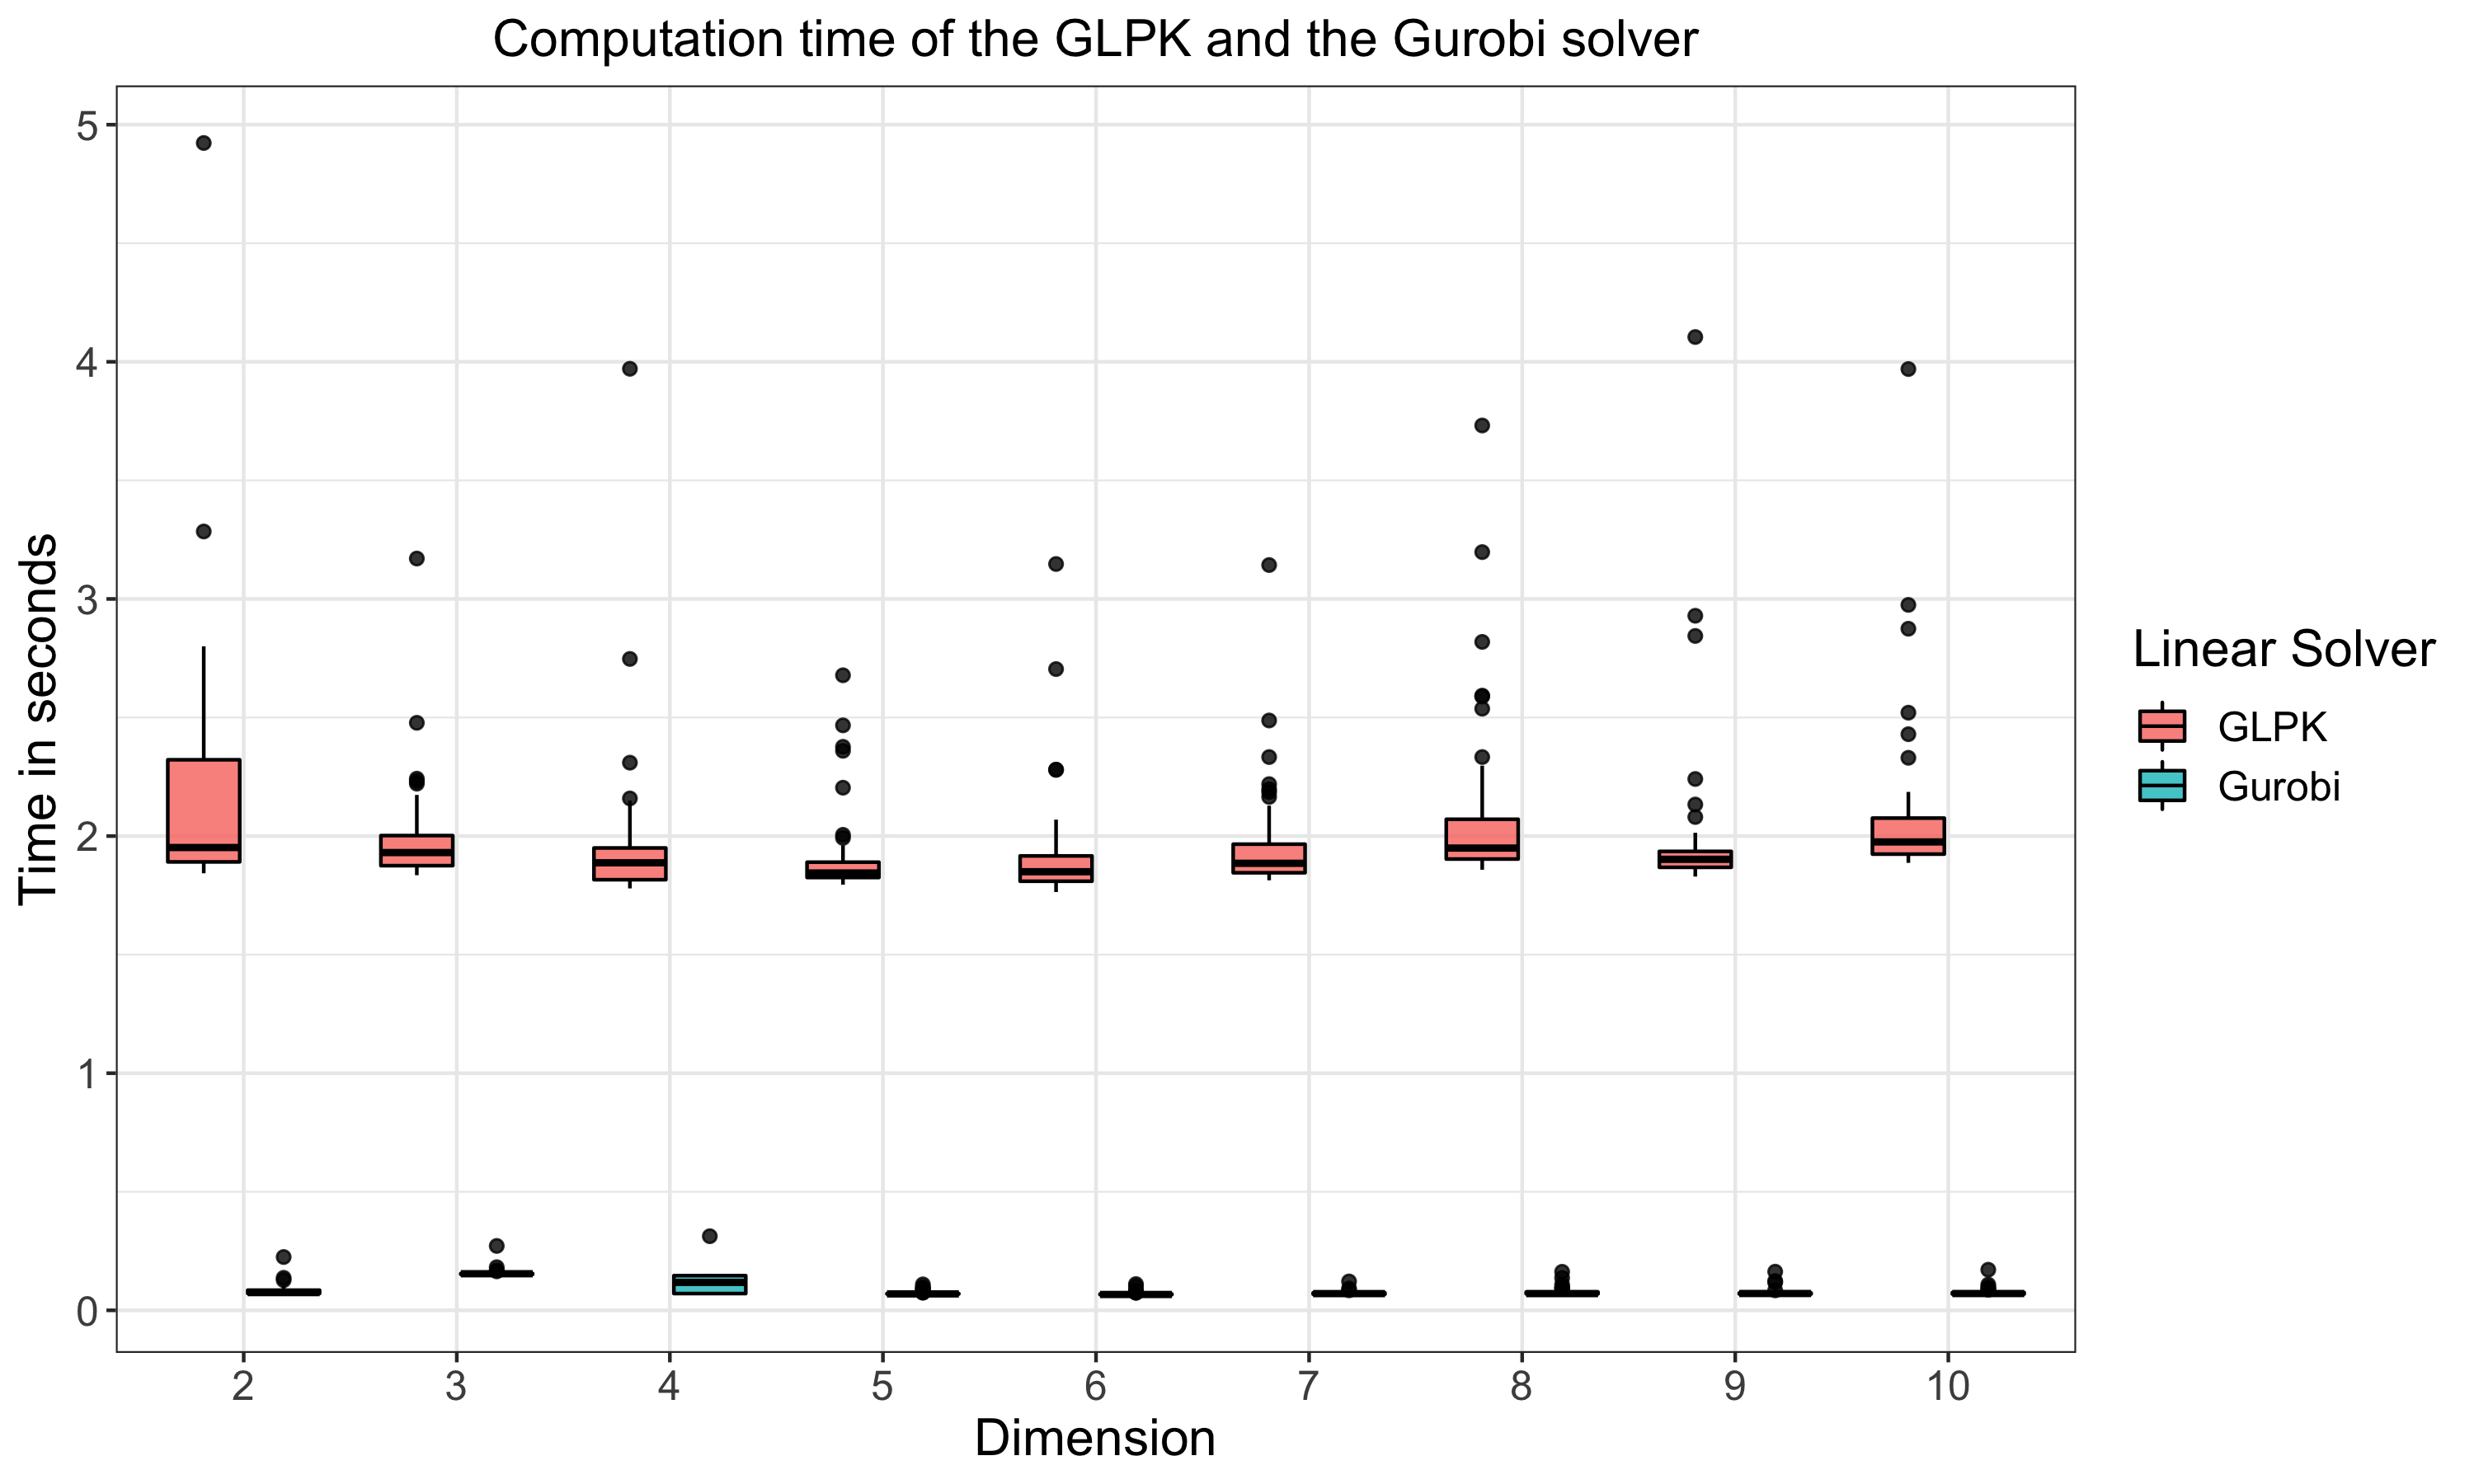
\includegraphics[width=1\textwidth]{boxplots_glpk_gurobi.jpg}% This is a *.eps file
 \end{center}
 \caption{Computation time of the GLPK linear solver (red) and the Gurobi linear solver (green) to solve the uniform/length-weighted edge-loss minimal problems in Algorithm 1. We perform experiments on $90$ data sets, 10 for each dimension 2-10, generated from the normal distribution. The horizontal axis is the dimension of the data set, and the vertical axis is the time it takes to solve an optimization problem. We observe that the Gurobi solver is consistently faster than the GLPK solver and that computation time seems fairly constant across dimension.}\label{fig:glpk_gurobi}
 \end{figure}

% % \begin{figure}[h!]
% % \begin{center}
% % 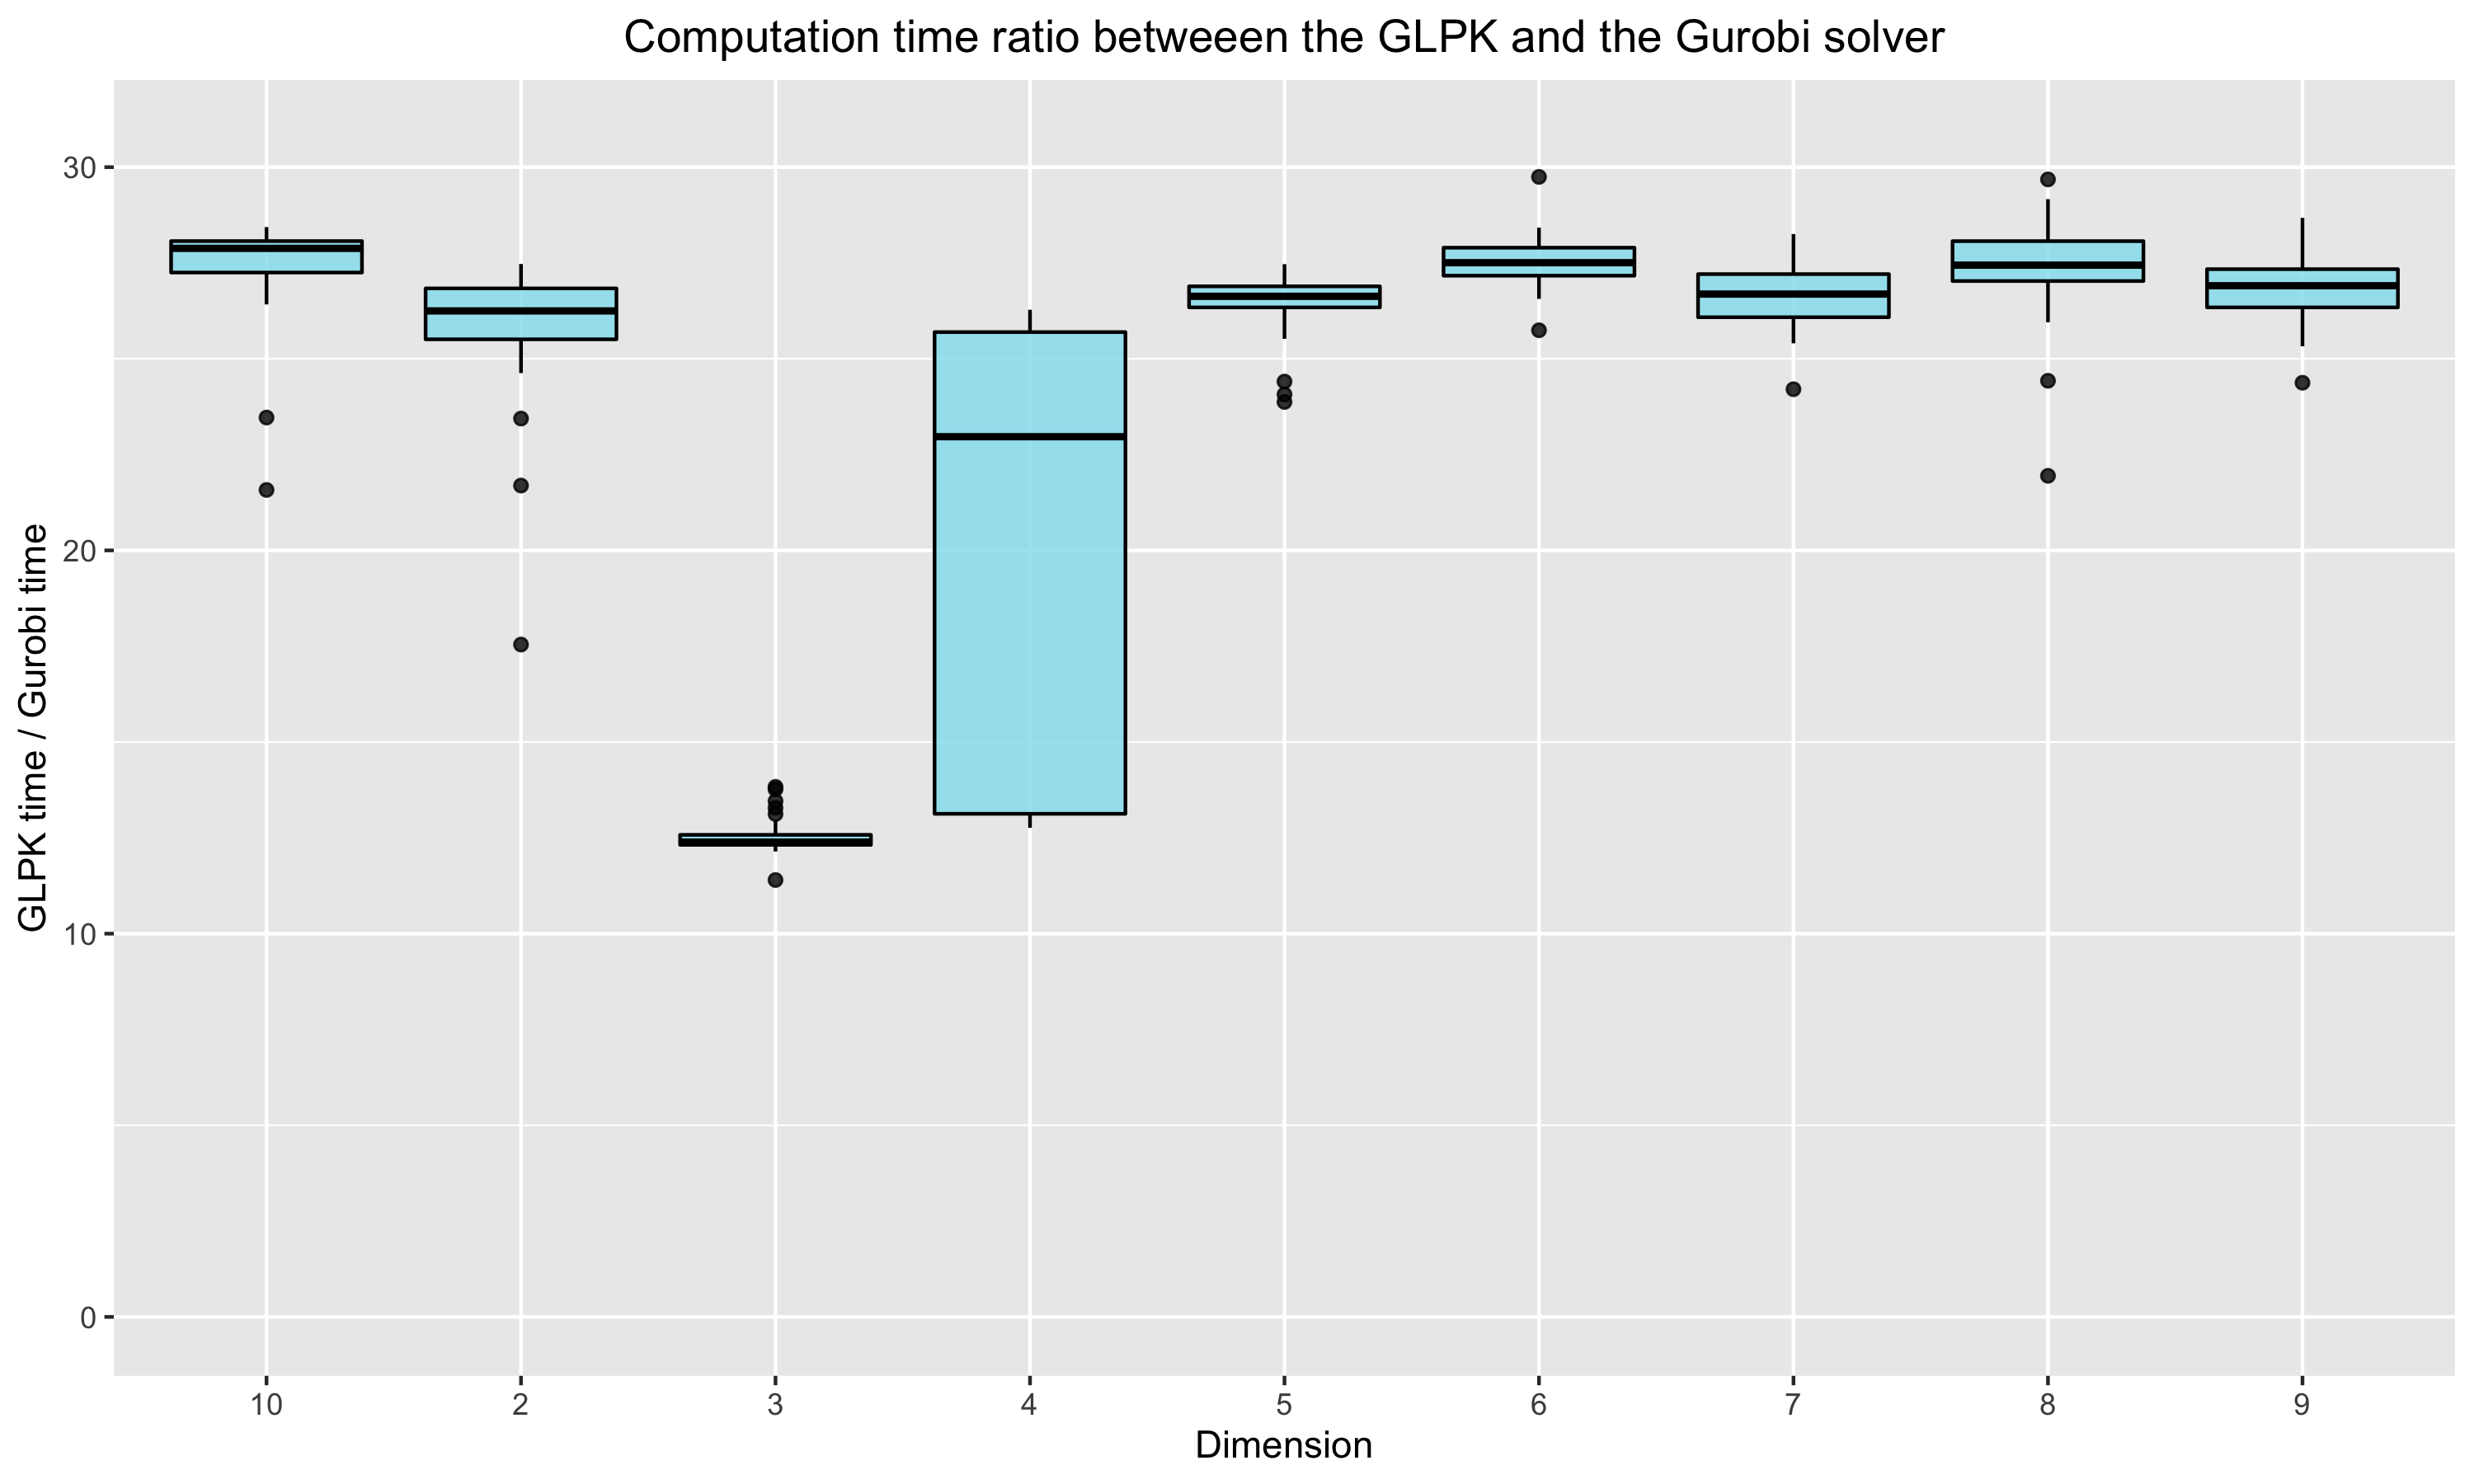
\includegraphics[width=1\textwidth]{figures/computationratio_glpk_gurobi.png}% This is a *.eps file
% % \end{center}
% % \caption{Computation time ratio of the GLPK and Gurobi linear solver. We observe that the Gurobi solver can be a lot faster than the GLPK solver.}\label{fig:glpk_gurobi}
% % \end{figure}


% section 6
\begin{figure}[h!]
\begin{center}
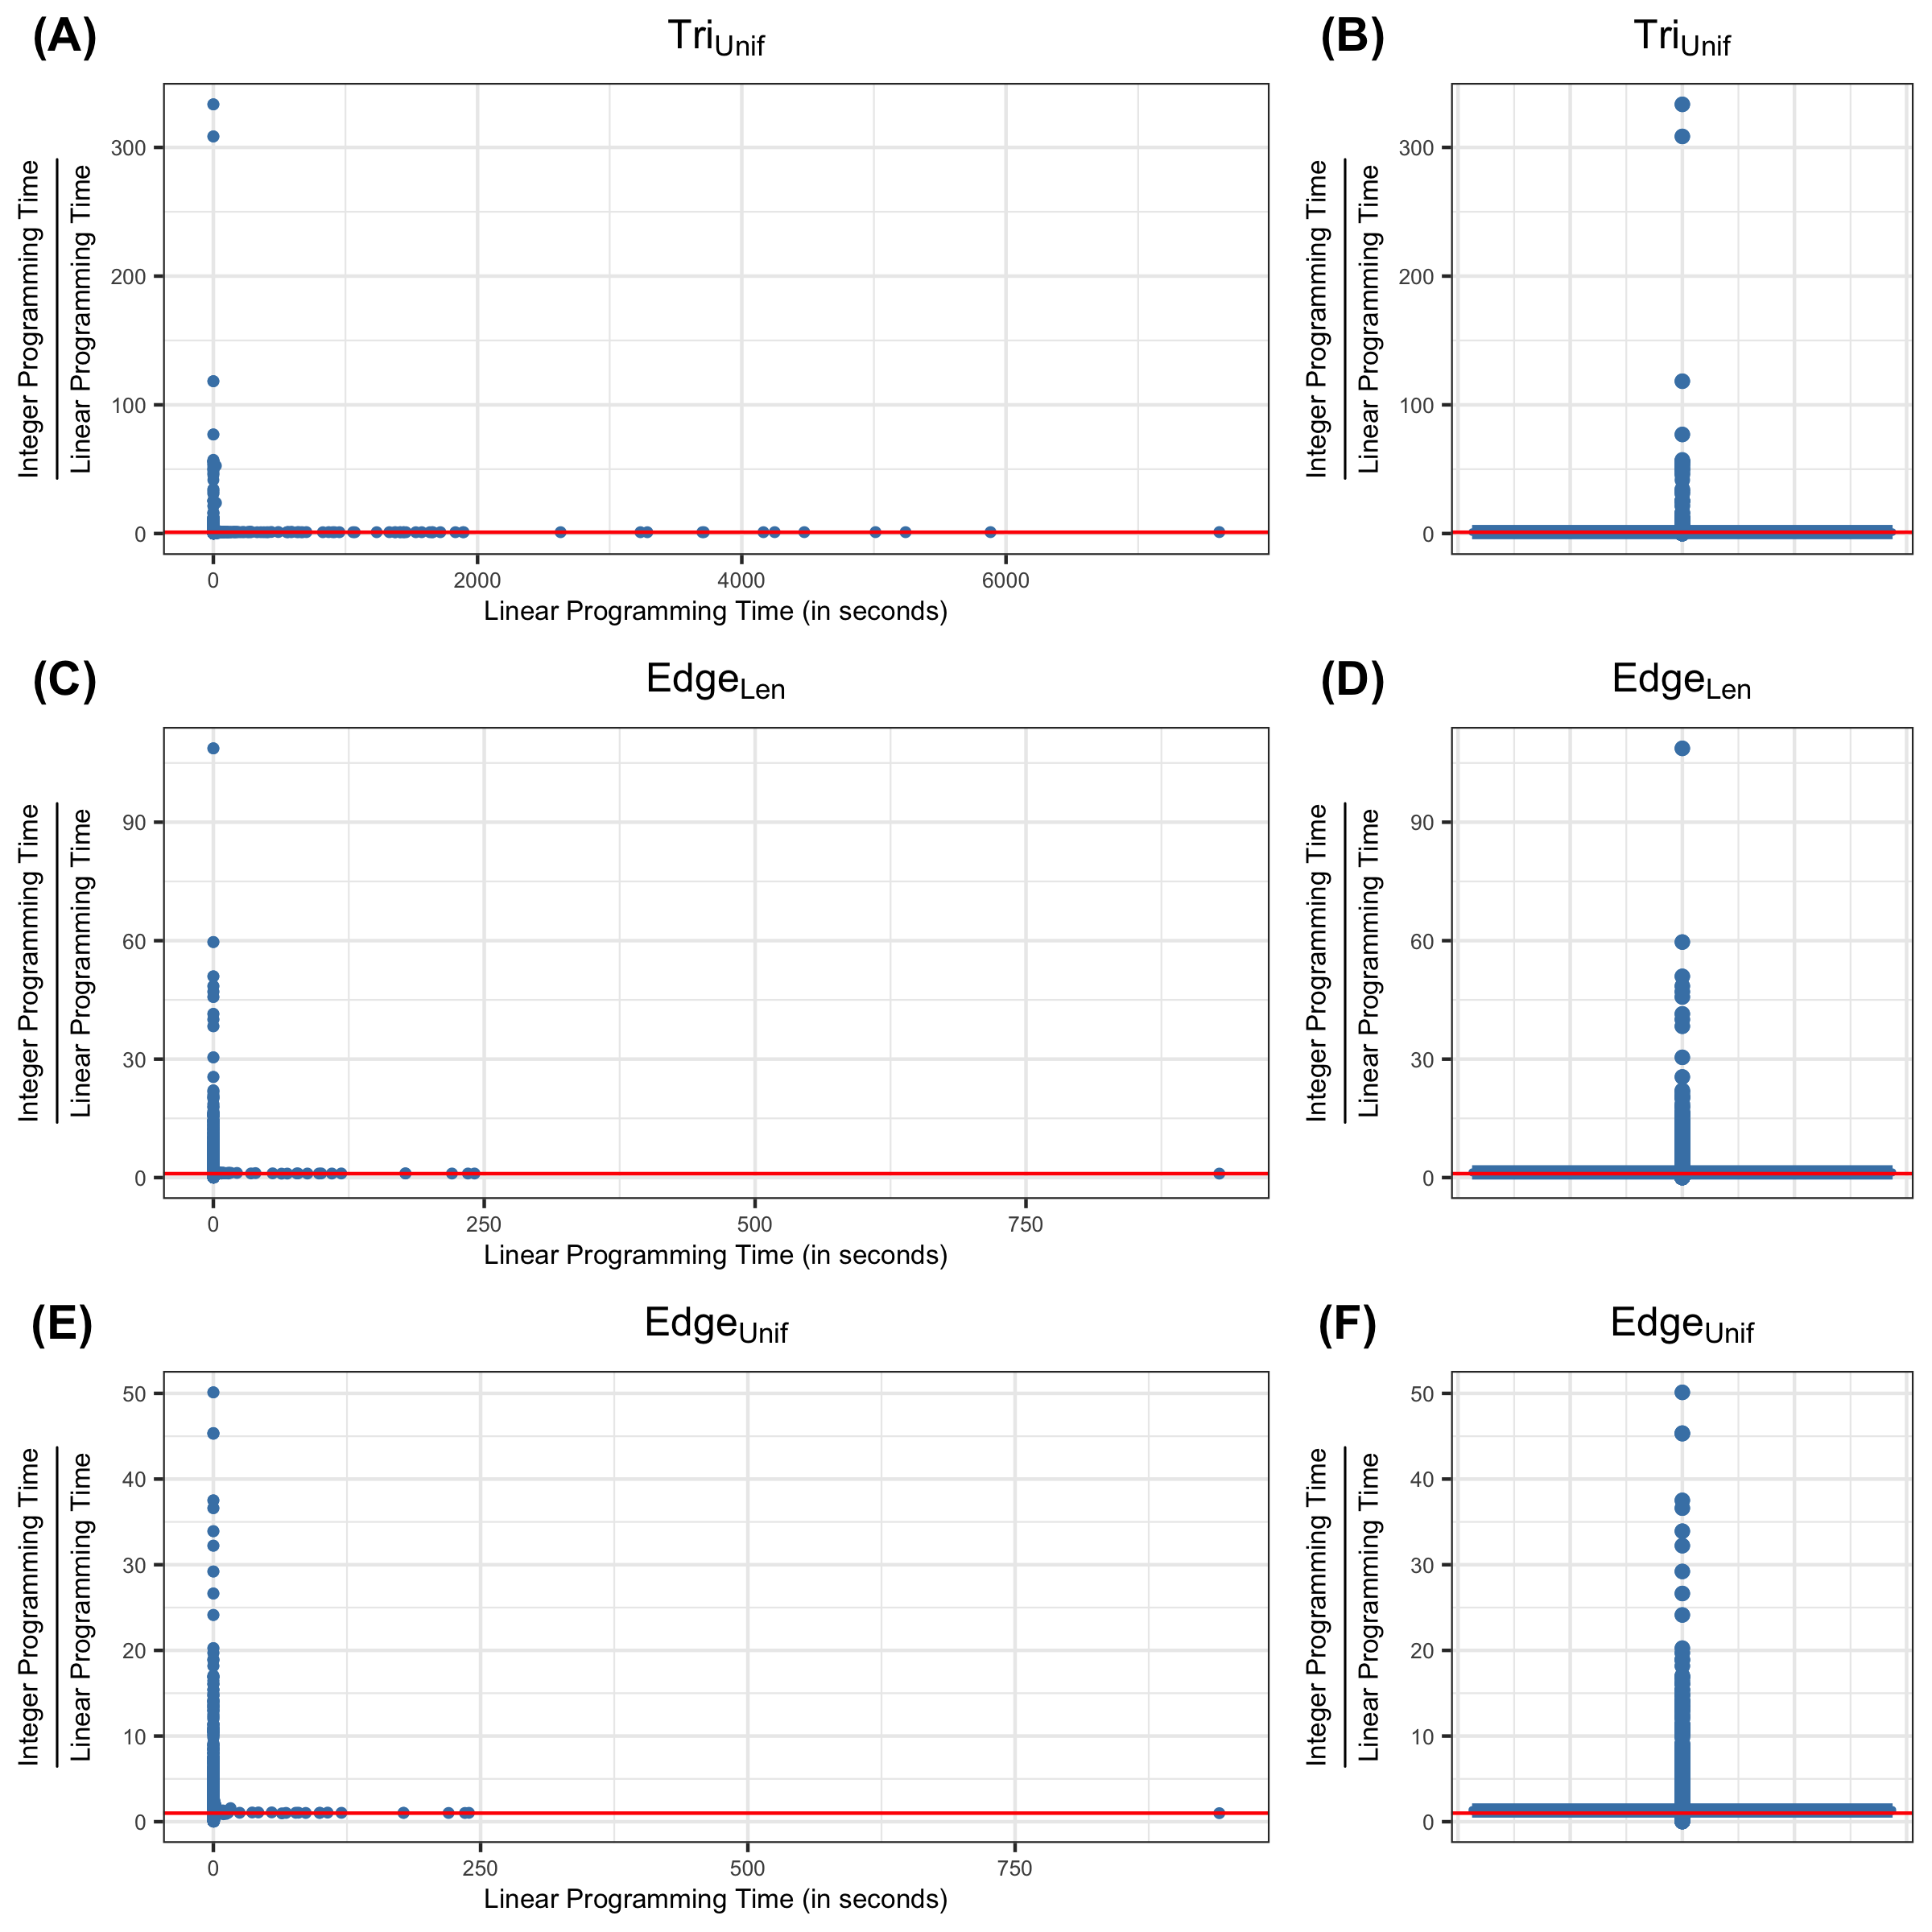
\includegraphics[width=\textwidth]{figures/IPvsLP.png}% This is a *.eps file
\end{center}
 \caption{
%  \GHP{Delete the phrase ``This figure shows the'' in every figure caption. }
 Ratio between the computation time of solving an integer programming problem Programs \ref{itm:tri_IU},\ref{itm:edge_IL}, \ref{itm:edge_IU} and the computation time of solving a linear programming problem Programs \ref{itm:tri_NIU},\ref{itm:edge_NIL}, \ref{itm:edge_NIU} for all the cycle representatives from data sets described in \se \ref{tab:realworldata} and \se \ref{tab:distributiondata}. Subfigures  \textbf{(A), (C), (E)} plot the data using scatter plots and subfigures  \textbf{(B), (D), (F)} show the same data using box plots. The vertical axis represents the ratio between the integer programming time and linear programming time of optimizing a cycle representative and the horizontal axis represents the computation time to solve the linear program. The red line in each subfigure represents the horizontal line $y=1$, where the time for each optimization is equivalent. As we can see from the box plots, the ratio between the computation time of integer programming and linear programming for most of the cycle representatives ($>50\%$) center around $1$.}\label{fig:lp_mip_ratio_df}
\end{figure}
% \begin{figure}[h!]
% \begin{center}
% 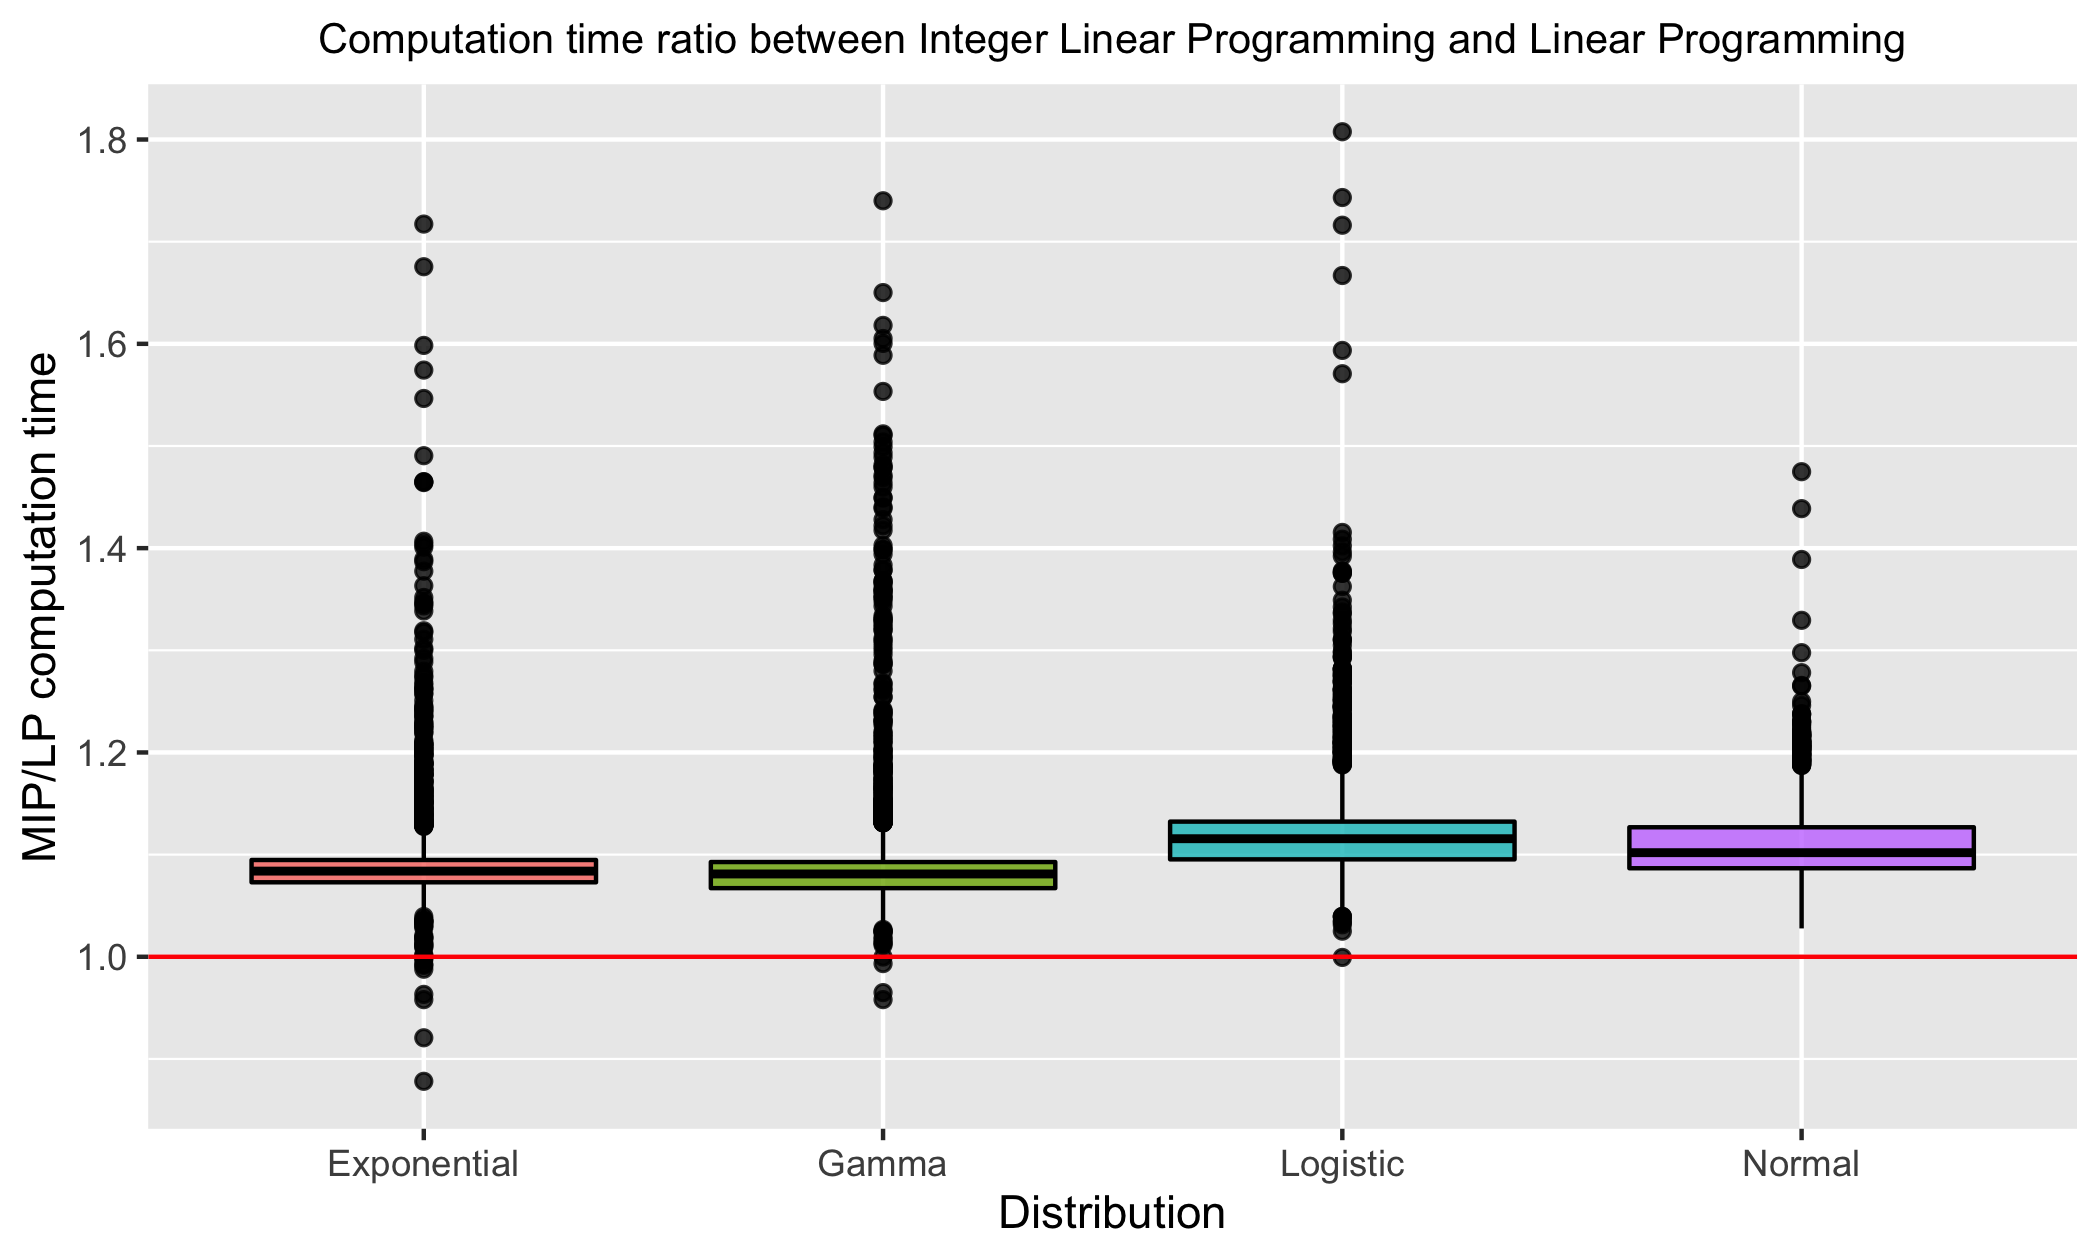
\includegraphics[width=0.8\textwidth]{figures/comptime_dist.png}% This is a *.eps file
% \end{center}
% \caption{Computation time ratio between integer programming and linear programming for randomly generated data sets. The x-axis is the distribution, and the y-axis is the ratio between the computation taken between requiring integer solutions and not requiring integer solutions. The red line marks the the value of 1. Linear programming was almost always faster than integer linear programming, although none of the displayed ratios exceed 2.0. }\label{fig:lp_mip_ratio_dist}
% \end{figure}

% delete legend 
% make x,y,title labels larger
\begin{landscape}
\begin{figure}[hbt!]
\begin{center}
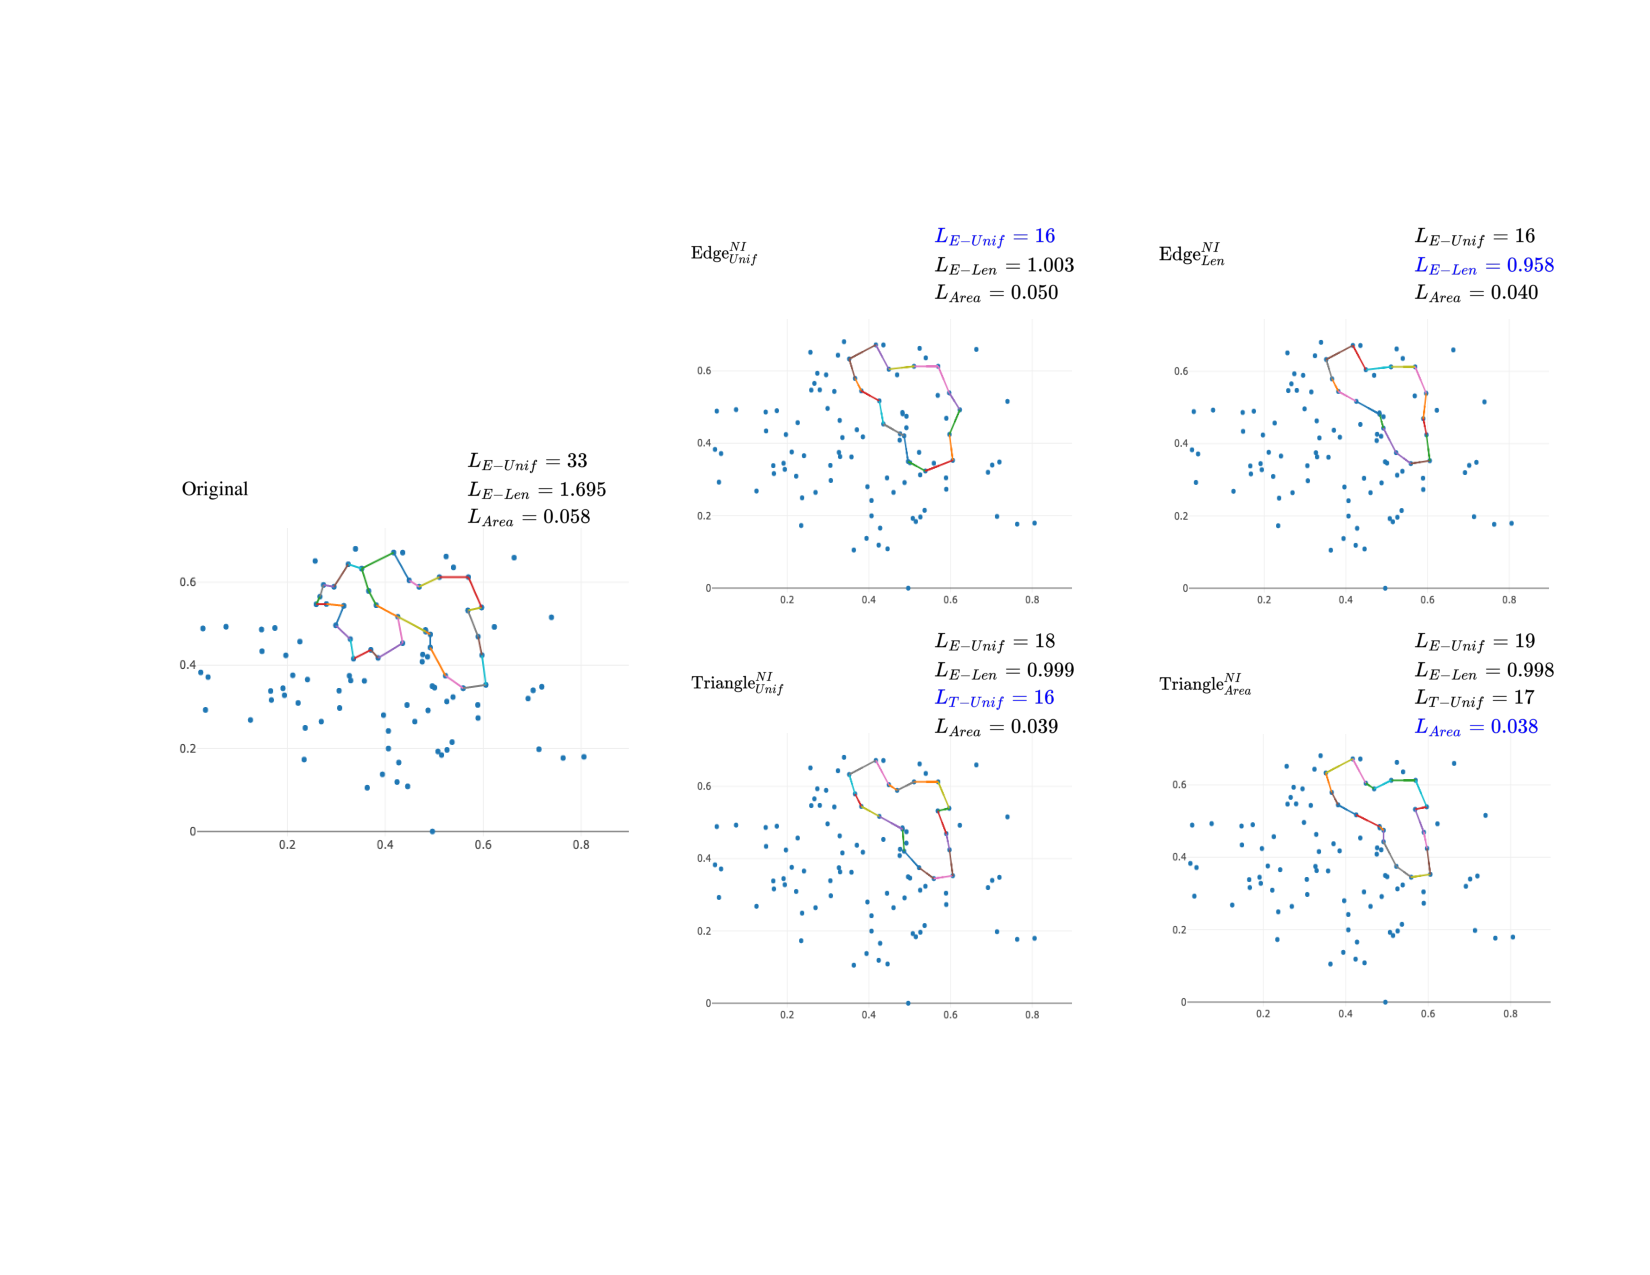
\includegraphics[width=\textwidth]{figures/examples.pdf}
\end{center}
\caption{Examples of different optimal cycles and cost against different loss functions using a point cloud of $100$ points with ambient dimension $2$ randomly drawn from a normal distribution. The upper left corner of each subfigure labels the optimization algorithm used to optimize the original cycle representative. The upper right corner of each subfigure records the different measures of the size of the optimal representative. Blue text represents the measure an algorithm sets out to optimize. 
}\label{fig:Examplesofeachoptimalcycles} 
\end{figure}
\end{landscape}
% \textbf{(A)} is the original cycle, \textbf{(B)} is the uniform-weighted minimal cycle, \textbf{(C)} is the length-weighted minimal cycle, \textbf{(D)} is the volume, \textbf{(E)} is the area optimal cycle.

% \vspace{0.1in}

% \begin{table}[hbt!]
%     \centering
%     \begin{tabular}{ |c || c |c |c |c |}
%  \hline
%  & Length & Edge  & Area & Volume  \\[0.5ex] 
%  \hline 
%  $X_{Orig}$ & 1.695 & 33  & 0.0576 &  -  \\\hline  

% $X_{Len}$ &  \textbf{0.0958} &  16  &  0.0398 &   -  \\\hline  
% $X_{Unif}$ & 1.003 & \textbf{16}   & 0.0496 &  -  \\\hline  

% $X_{Area}$ &   0.998  & 19  & \textbf{0.038 }& 17  \\  \hline
% $X_{Vol}$ &   0.999  & 18    & 0.0391 & \textbf{16} \\ \hline

% \end{tabular}
% \caption{Summary of the example in Figure \ref{fig:volumeExample}}
% \label{tab:data}
% \end{table}

\begin{figure}[h!]
\begin{center}
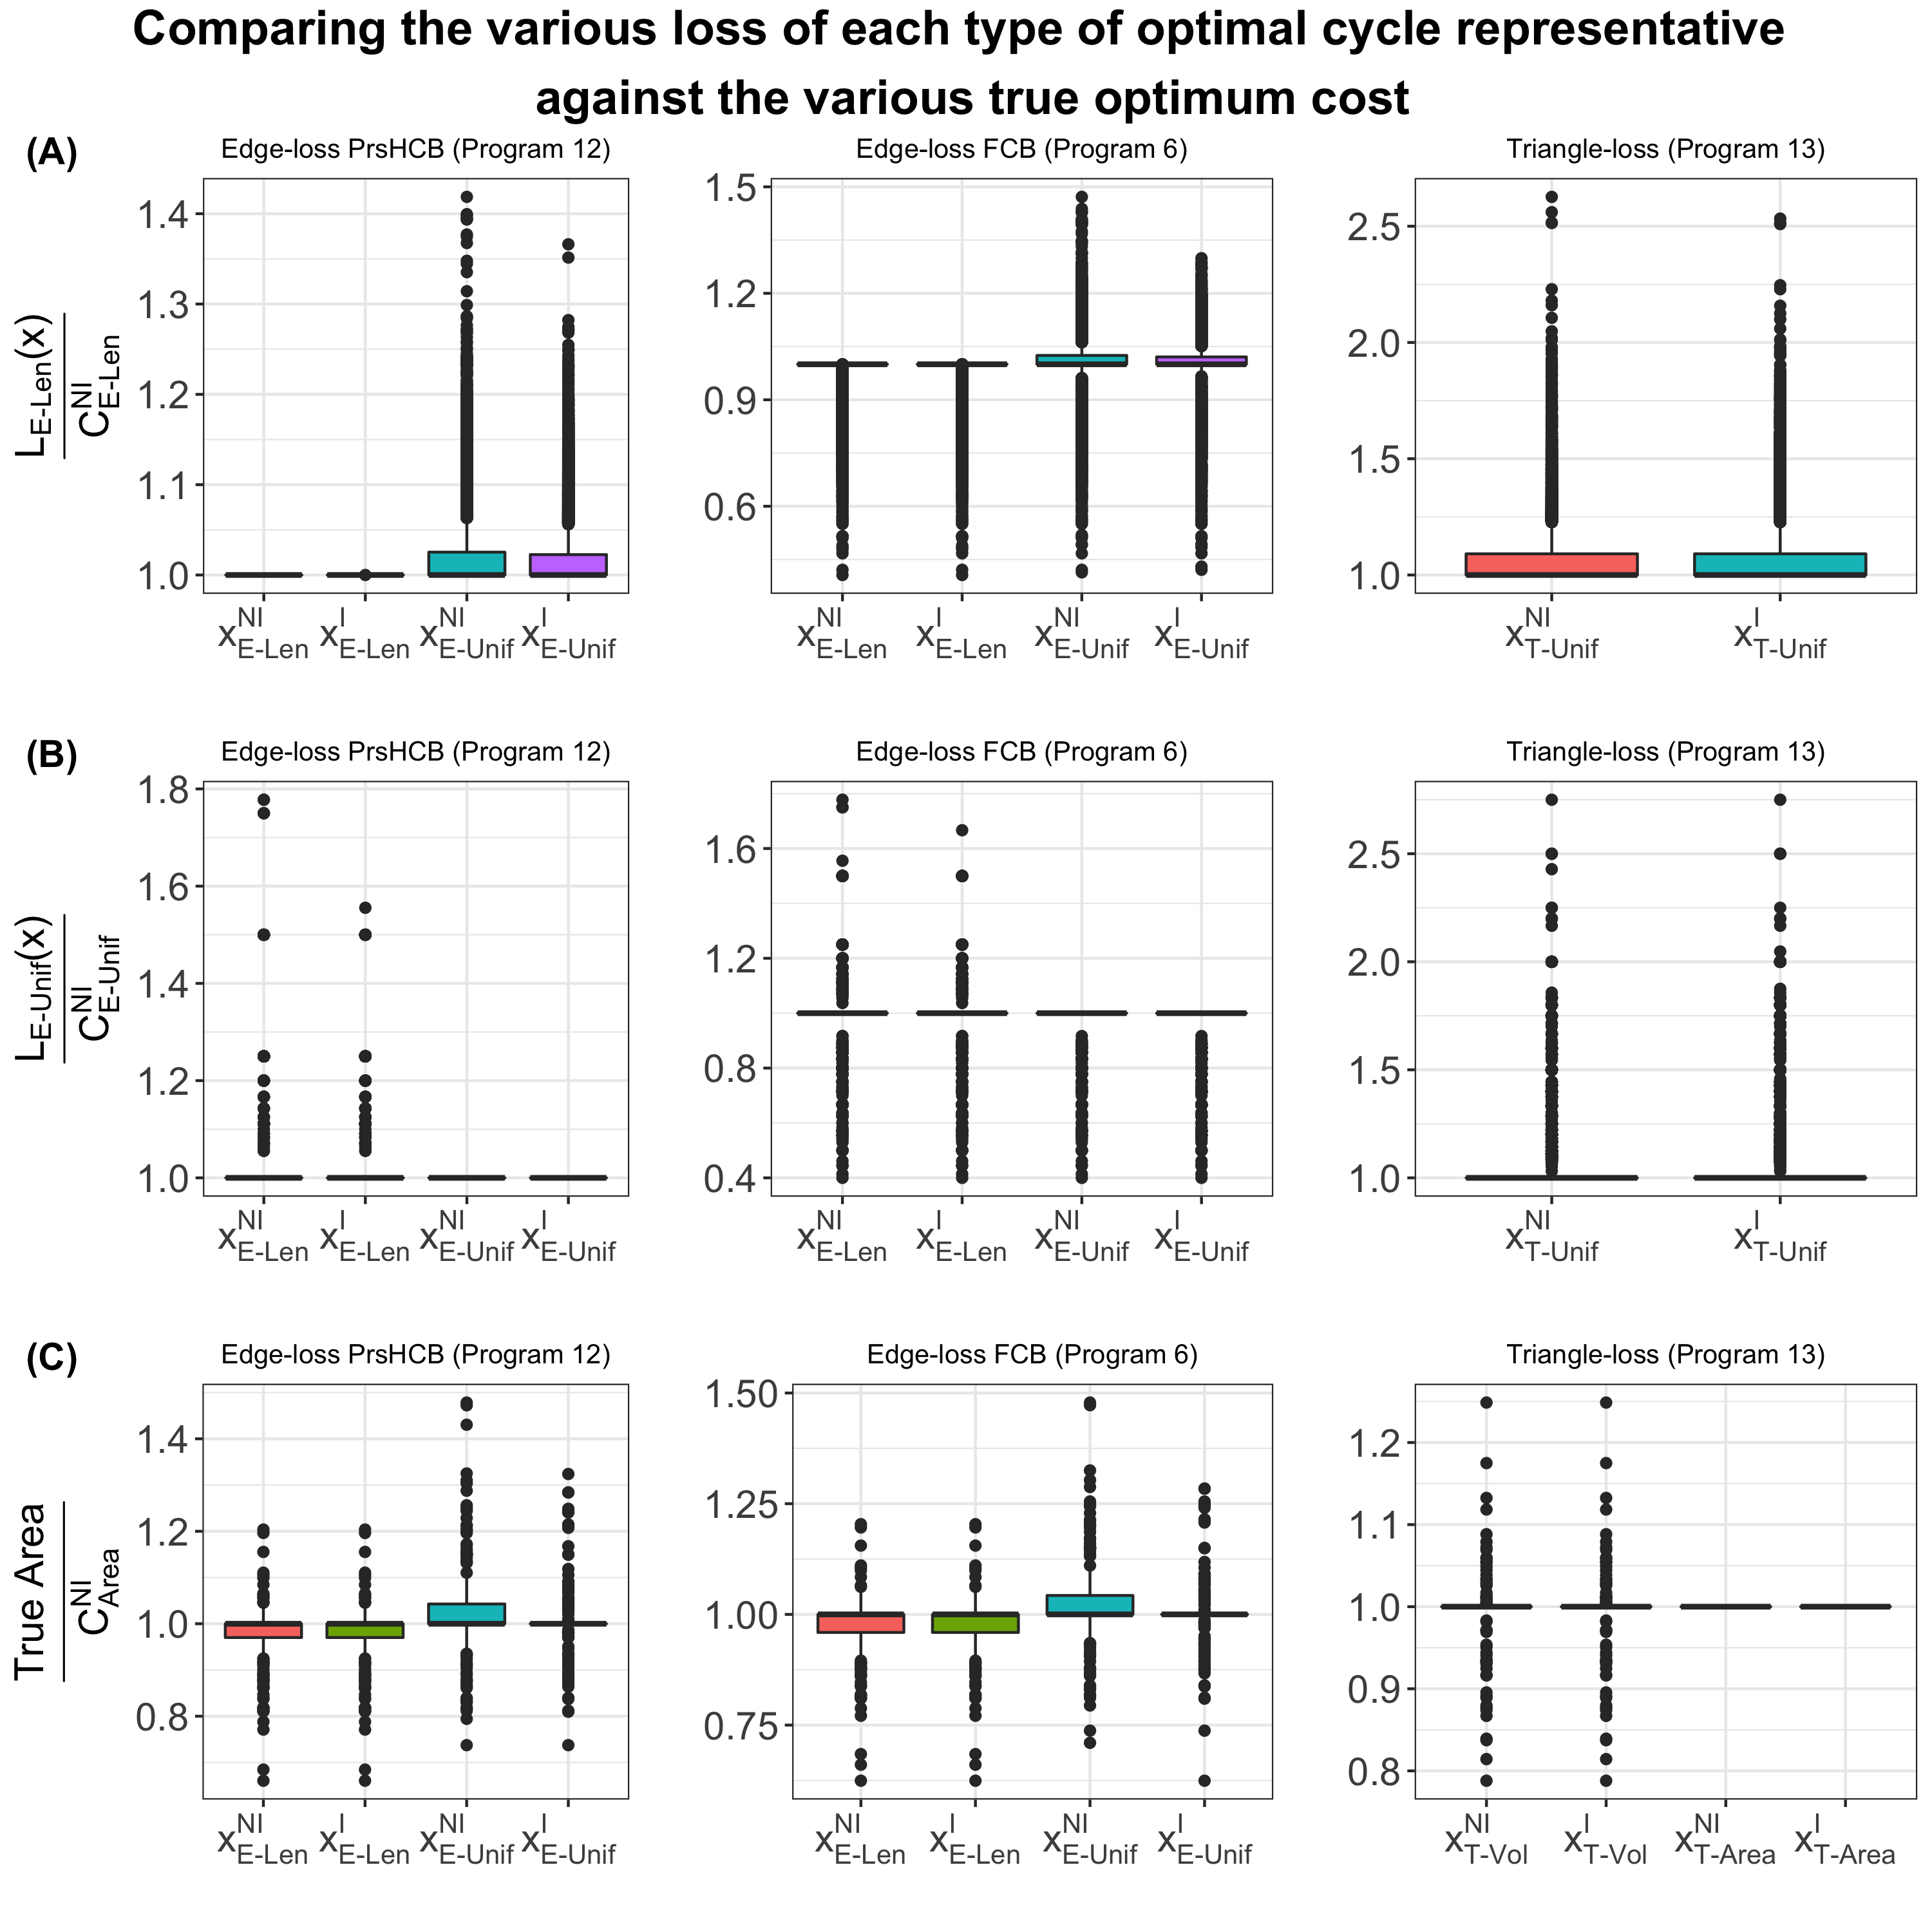
\includegraphics[width=\textwidth]{figures/length_area_edge.png}
\end{center}
\caption{Box plots of the ratios between (\textbf{A}) $L_{E\text{-}Len}(\optimalrep_\bullet^\bullet)$ and $C_{E\text{-}Len}$,  \textbf{(B)} $L_{E\text{-}Unif}(\optimalrep_\bullet^\bullet)$ and $C_{E\text{-}Unif}$, and  \textbf{(C)} $L_{T\text{-}Area}(\optimalrep_\bullet^\bullet)$ and $C_{T\text{-}Area}$. 
The horizontal axis is the type of optimal representative, $\optimalrep_\bullet^\bullet$, and the vertical axis is the ratio between the loss of each type of optimal representative over the actual cost of the optimal representative of the same loss function, i.e. the $\setofpersistenthcyclebases$ cycles which are solutions to Programs \ref{itm:edge_NIU}, \ref{itm:edge_NIL}, \ref{itm:tri_NIA}.
In \se \ref{coefficient}, we discussed that the optimum cost is the same whether we require an integer solution or not for essentially all solutions for \pr \eqref{eq:edgelossgeneral}, \pr \ref{eq:escolarargmin}, and the uniform-weighted triangle-loss method, resulting in two columns in the first two rows having ratio 1. The data used in \textbf{(A)} and \textbf{(B)} aggregate over all data described in \ref{sec: realworlddata} and \ref{sec: randompointclouds}. The data used in \textbf{(C)} aggregate the $190$ cycle representatives from $10$ point clouds from a normal distribution with ambient dimension of $2$. True area represents the total area enclosed by the representative, while $C_{Area}\NI$ represents the area of the area-weighted triangle-loss optimal cycle minimizing \ref{itm:tri_NIA}. We observe that some edge-loss optimal cycles and triangle-loss optimal cycles requiring integral solutions have an area smaller than that of the area-weighted triangle-loss optimal cycle. Refer to Figure \ref{fig:areaExample} and \se  \ref{sec:comparing optimal generators against different loss functions} to see why this may happen. 
% In addition to $\optimalrep_{Area}\NI = \optimalrep_{Area}\I$ for corresponding cycle representatives in all experiments, so too are $\optimalrep_{Len}\NI = \optimalrep_{Len}\I$.
}
 \label{fig:lengthcocmpare}
\end{figure}


 %\begin{figure}[h!]
%\begin{center} 
%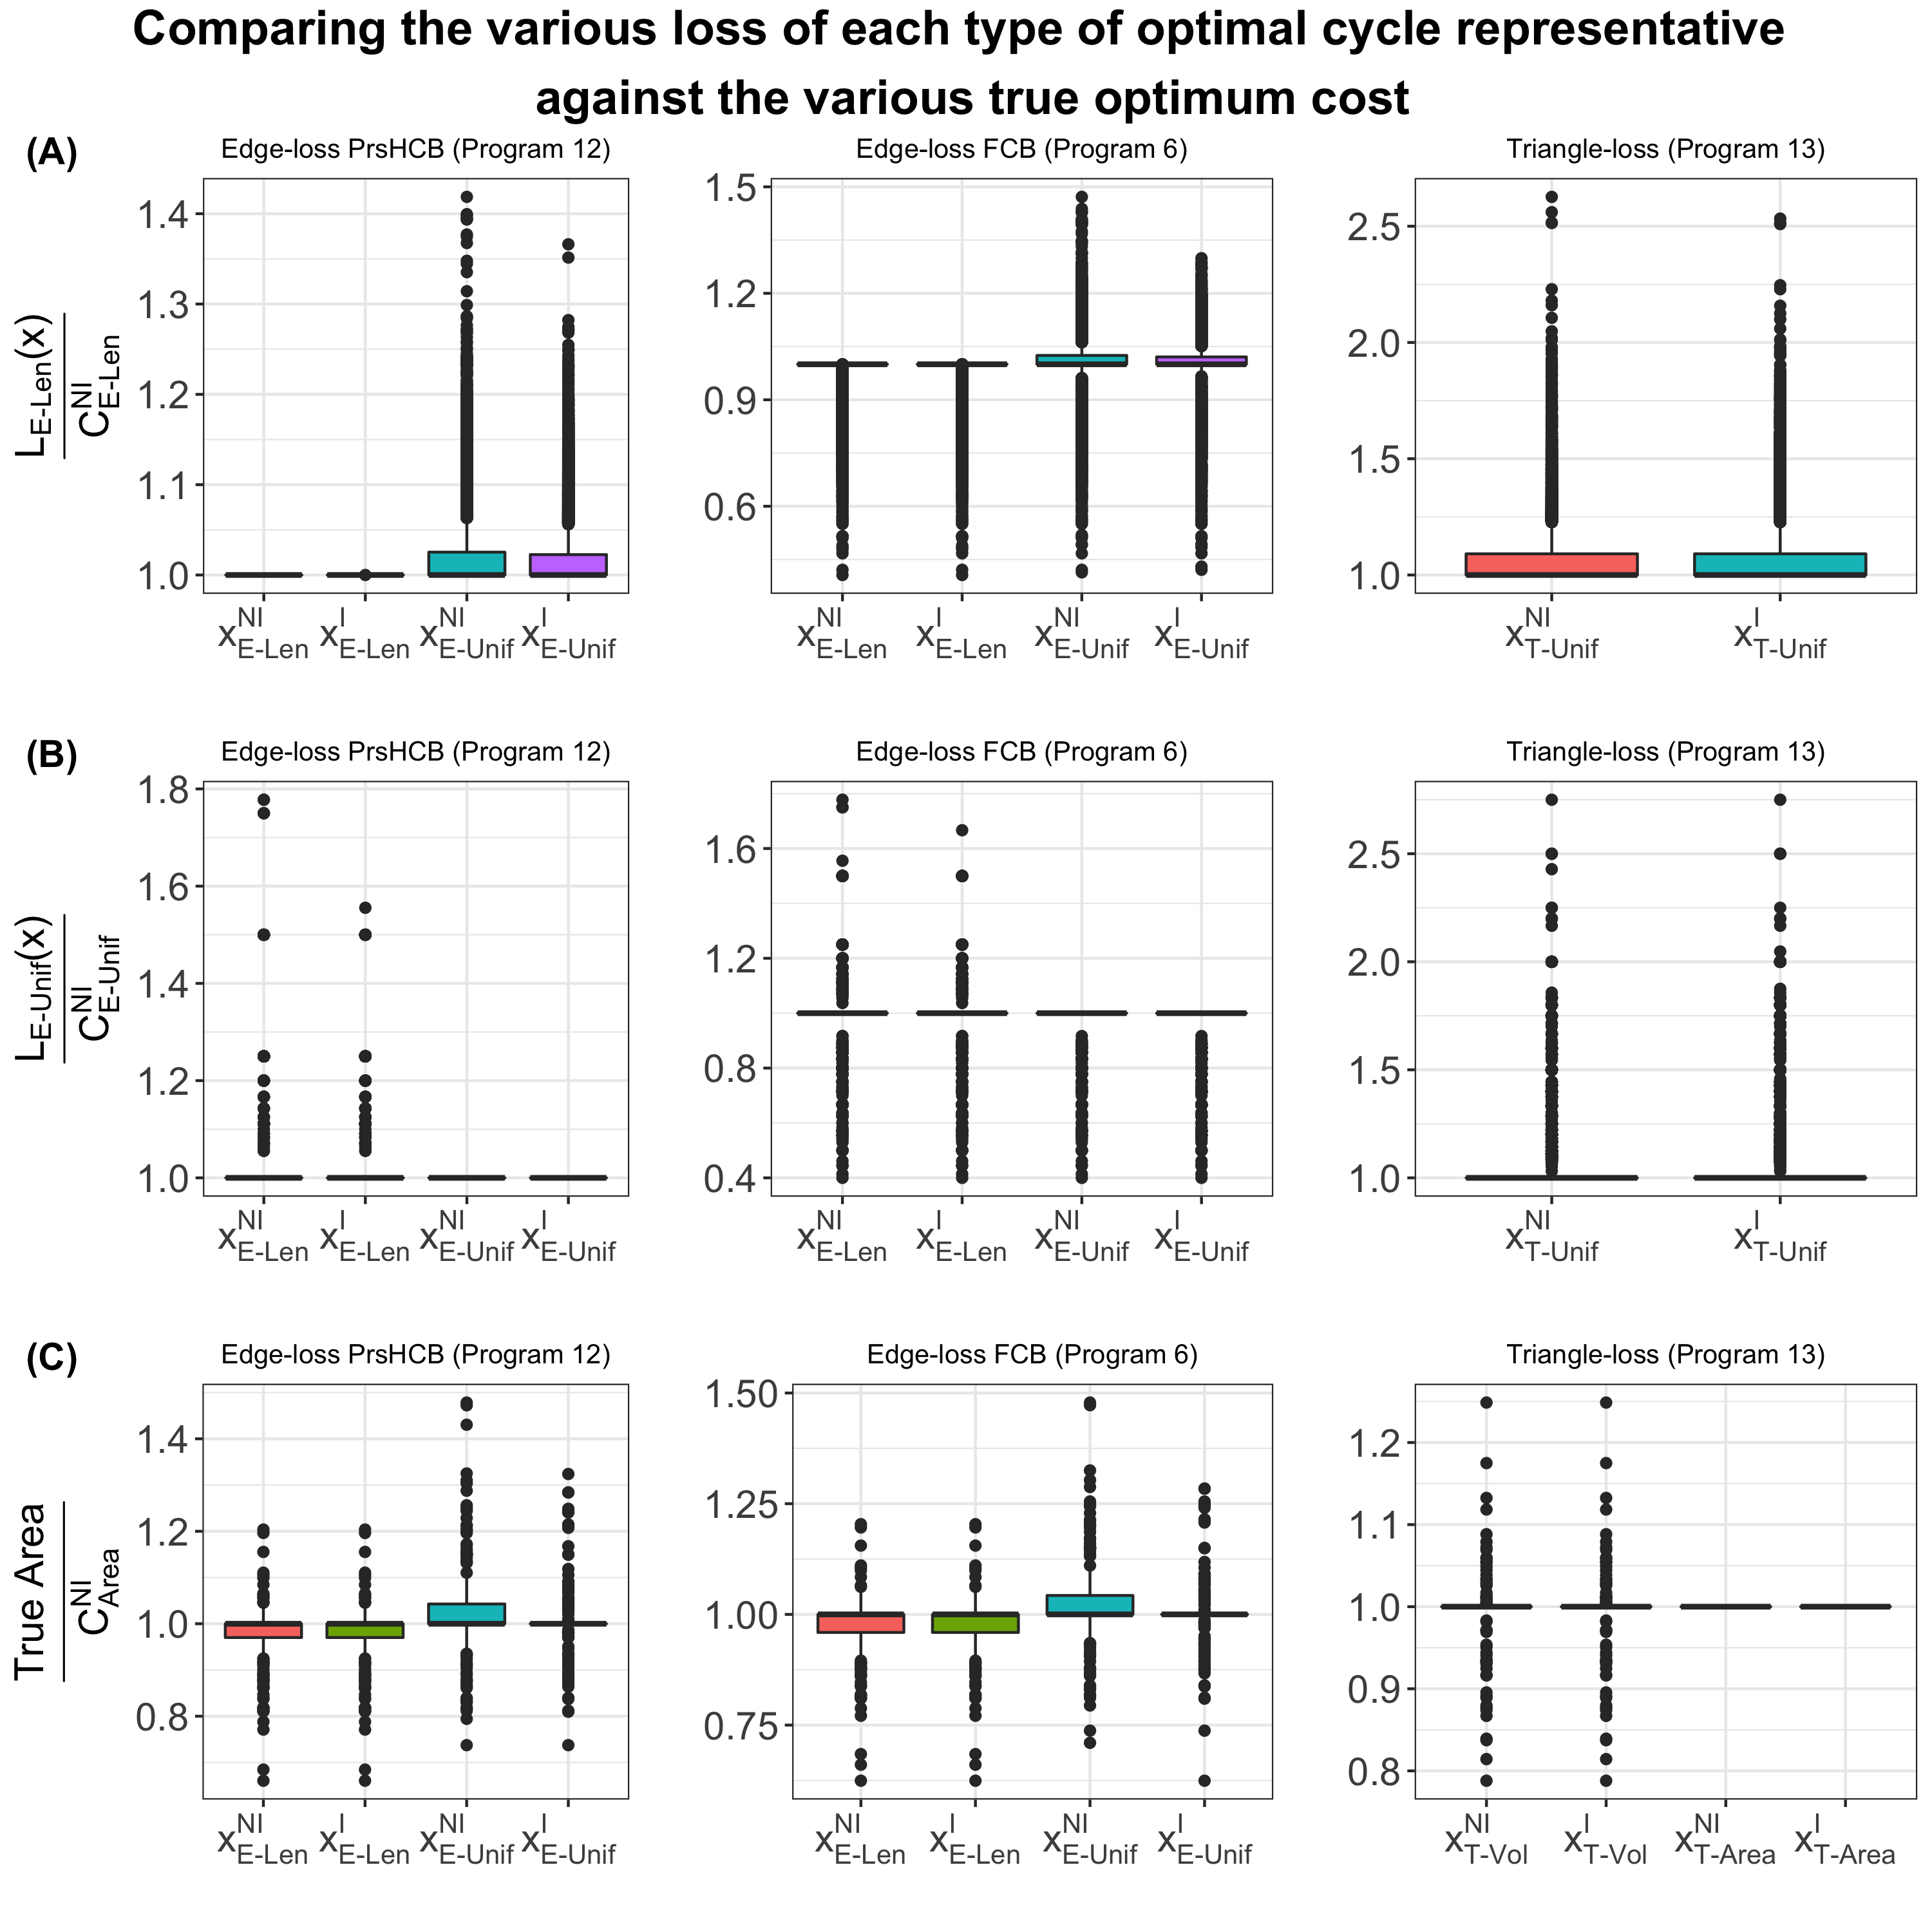
\includegraphics[width=\textwidth]{figures/length_area_edge.png}
%\end{center}
%\caption{Box plot comparing the enclosed area of each type of optimal cycle representative against the optimum area-weighted volume optimal cost. These data aggregate $190$ cycle representatives from $10$ point clouds from a normal distribution with ambient dimension of $2$. True area represents the total area enclosed by the representative, while $C_{Area}\NI$ represents the area of the area-weighted volume optimal cycle minimizing \ref{eq:LP-Area}. We observe that some uniform/length-weighted optimal cycles have an area smaller than that of the area-weighted volume optimal cycle. Refer to Figure \ref{fig:areaExample} to see why this may happen. In addition to $\optimalrep_{Area}\NI = \optimalrep_{Area}\I$ for corresponding cycle representatives in all experiments, so too are $\optimalrep_{Len}\NI = %\optimalrep_{Len}\I$\LZ{Remove, right??}}\label{fig:areacompare}
%\end{figure}

\begin{figure}[h!]
\begin{center}
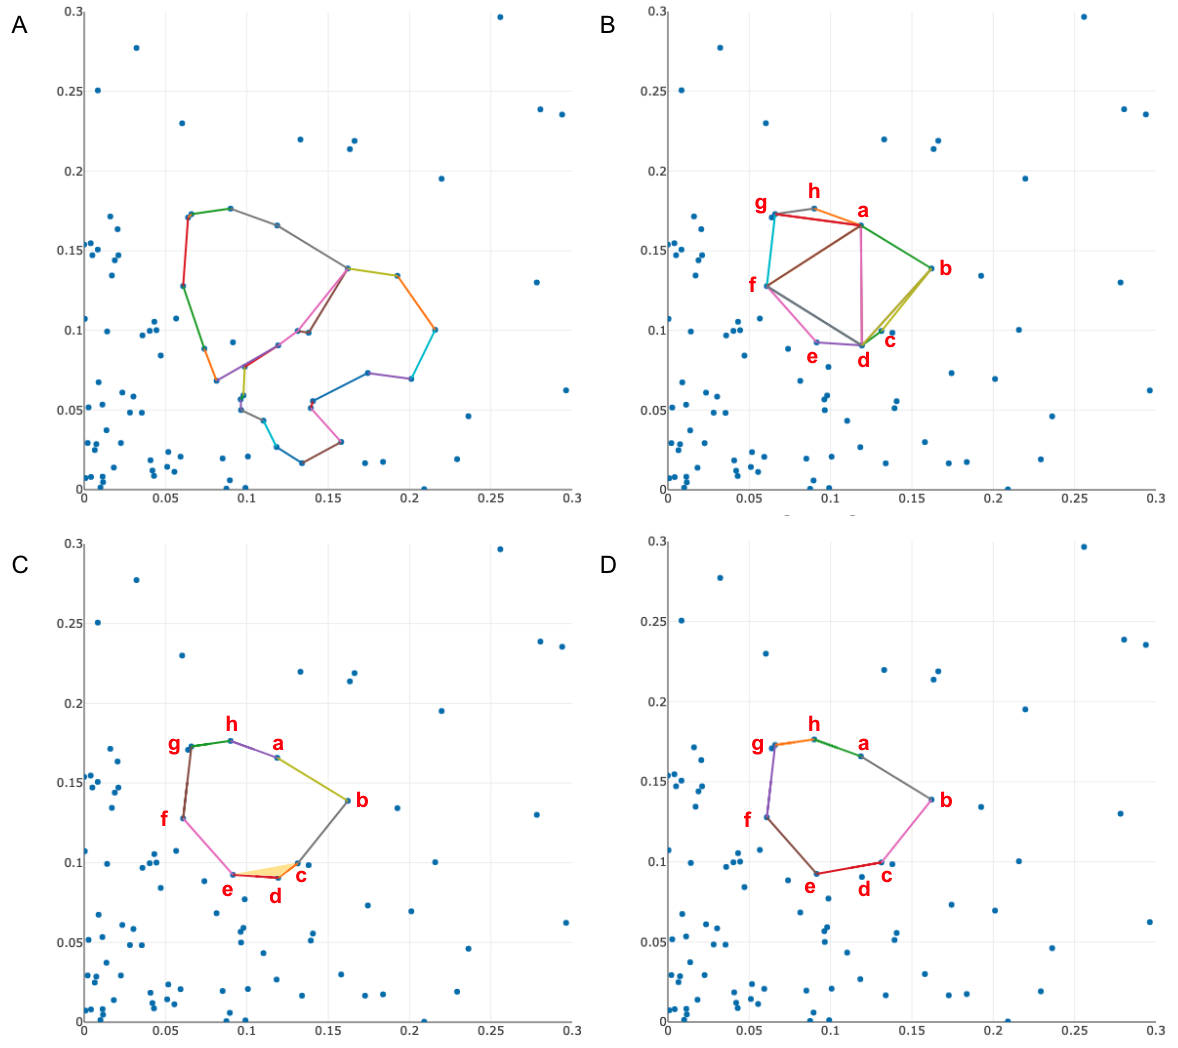
\includegraphics[width=15cm]{figures/areaExample4-2.png}
\end{center}
\caption{An example illustrating when the area enclosed by the triangle-loss area-weighted optimal cycle, solution to \pr \ref{itm:tri_NIA}, can be larger than the area enclosed by the edge-loss length-weighted minimal cycle, solution to \pr \ref{itm:edge_NIL}. \textbf{(A)} is the original cycle of a representative point cloud in $\mathbb{R}^2$ drawn from the normal distribution, \textbf{(B)} is the area-weighted optimal cycle triangulated based on the 2-simplices identified by nonzero entries in the coefficient vector $\volvec$, \textbf{(C)} is the area-weighted minimal cycle, \textbf{(D)} is the length-weighted minimal cycle. The yellow shaded area in \textbf{(C)} marks the difference in enclosed area by the area-weighted and length-weighted minimal cycle representatives. %The area-weighted volume optimal cycle contains the extra 2-simplex $[c,d,e].$
Constraint Equation \eqref{obacond1} specifies that the area-weighted optimal cycle must contain the 2-simplex born at the death time of the cycle. Therefore, this cycle must contain $\{a,d,f\}$ because it was born at the death time, and in fact, it contains both  $\{a,d,f\}$ and  $\{a,b,d\}$. The length-weighted minimal cycle does not have this constraint, and as such, can result in a smaller area. %\LL{Updated 0314}
%To get the length-weighted optimal cycle from the area-weighted volume optimal cycle, we still need to add the $2$-simplex $[c,d,e]$, which will increase the area-weighted volume, but will decrease the enclosed area. \LZ{I rephrased the previous sentence as: The length-weighted optimal cycle adds the $2$-simplex $[c,d,e]$ to the area-weighted volume optimal cycle, which increases the area-weighted volume but decreases the enclosed area....but now I don't think I understand the last part. The length-weighted does not care about the 2-simplices enclosed.}\CT{maybe: Our area-weighted volume optimal cycle differs from the length-weighted optimal cycle by the 2-simplex $[c,d,e]$. Although adding this 2-simplex would decrease the area of the cycle representative, it would increase our measured cost $||W\optimalrep||_1$.} 
}\label{fig:areaExample}
\end{figure}


\begin{figure}[h!]
\begin{center}
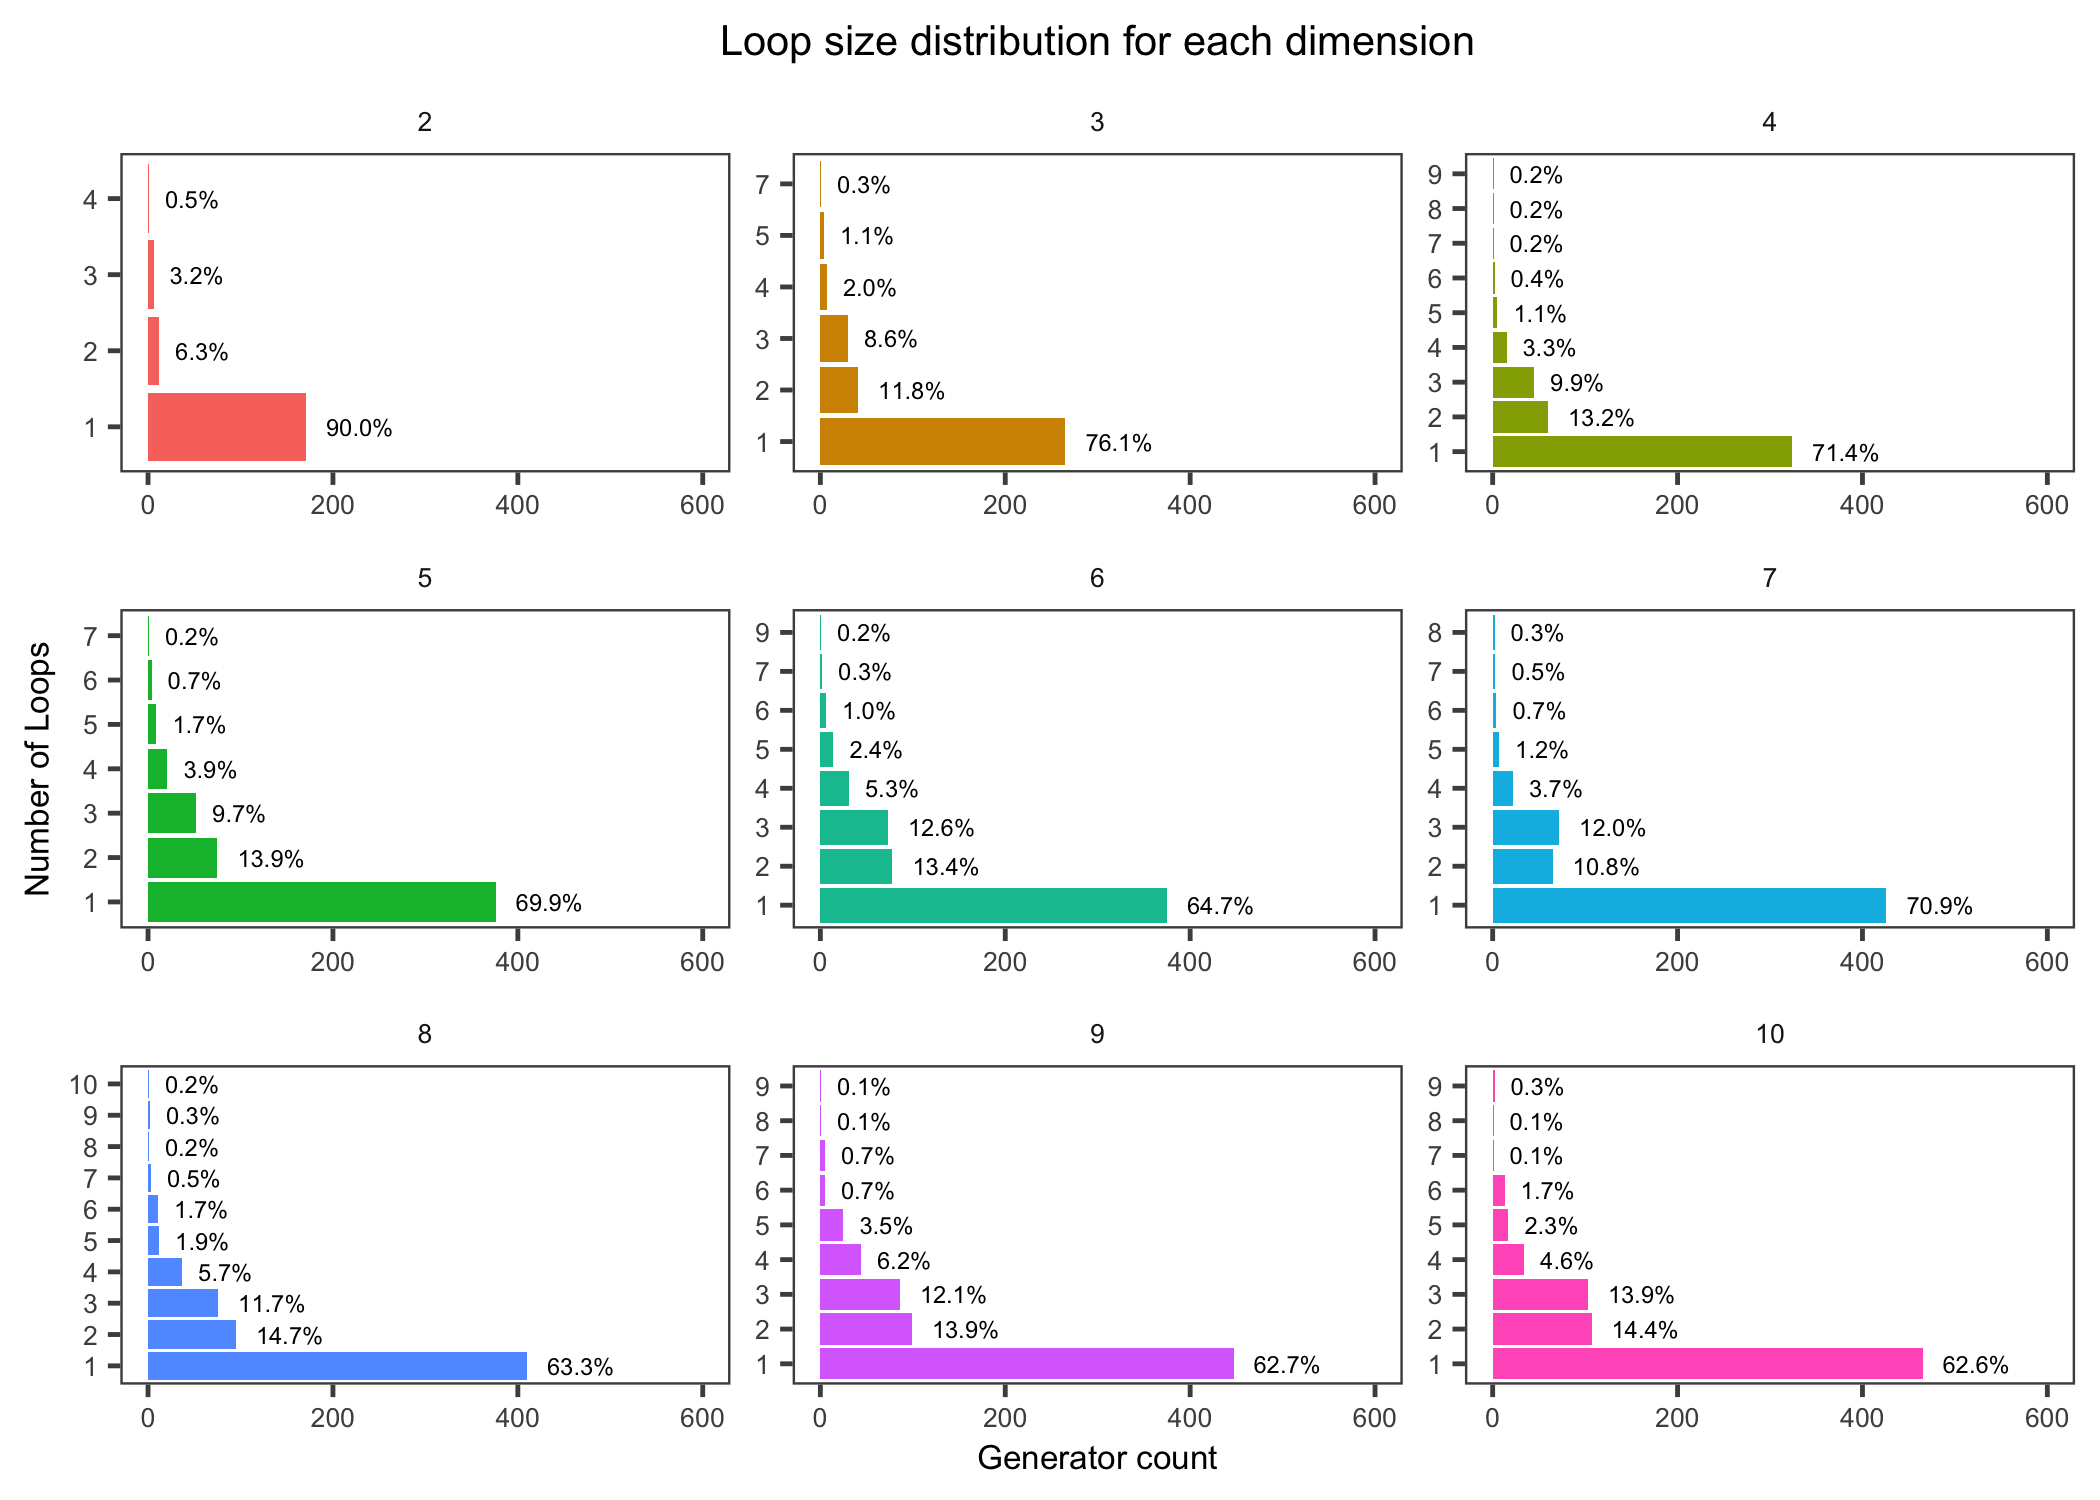
\includegraphics[width=\textwidth]{figures/loopsBreakdown.png}
\end{center}
\caption{%\GHP{First betti number of the support of $\optimalrep$, for various 1-d cycle representatives $\optimalrep$ (equivalently, the nullity of the column submatrix $[\partial_1][:, S]$, where $S = \{i : \optimalrep_i \neq 0\}$ is the support of $\optimalrep$)}\LL{Thanks for this definition, Greg! We added it to the results section 6.8. Should we also keep it here?}  
Number of loops in the original cycle representatives of each dimension (subfigure title) in the $360$ randomly generated distribution data sets. The horizontal axis is the number of representatives and the vertical axis is the number of loops in the original representative. We observe that original cycle representatives can have up to 10 loops in higher dimensions, and in general, it is not uncommon to find an original representative with multiple loops.} \label{fig:loopsbreakdown}
\end{figure} 
% 

% \begin{landscape}
\begin{figure}[h!]
\begin{center}
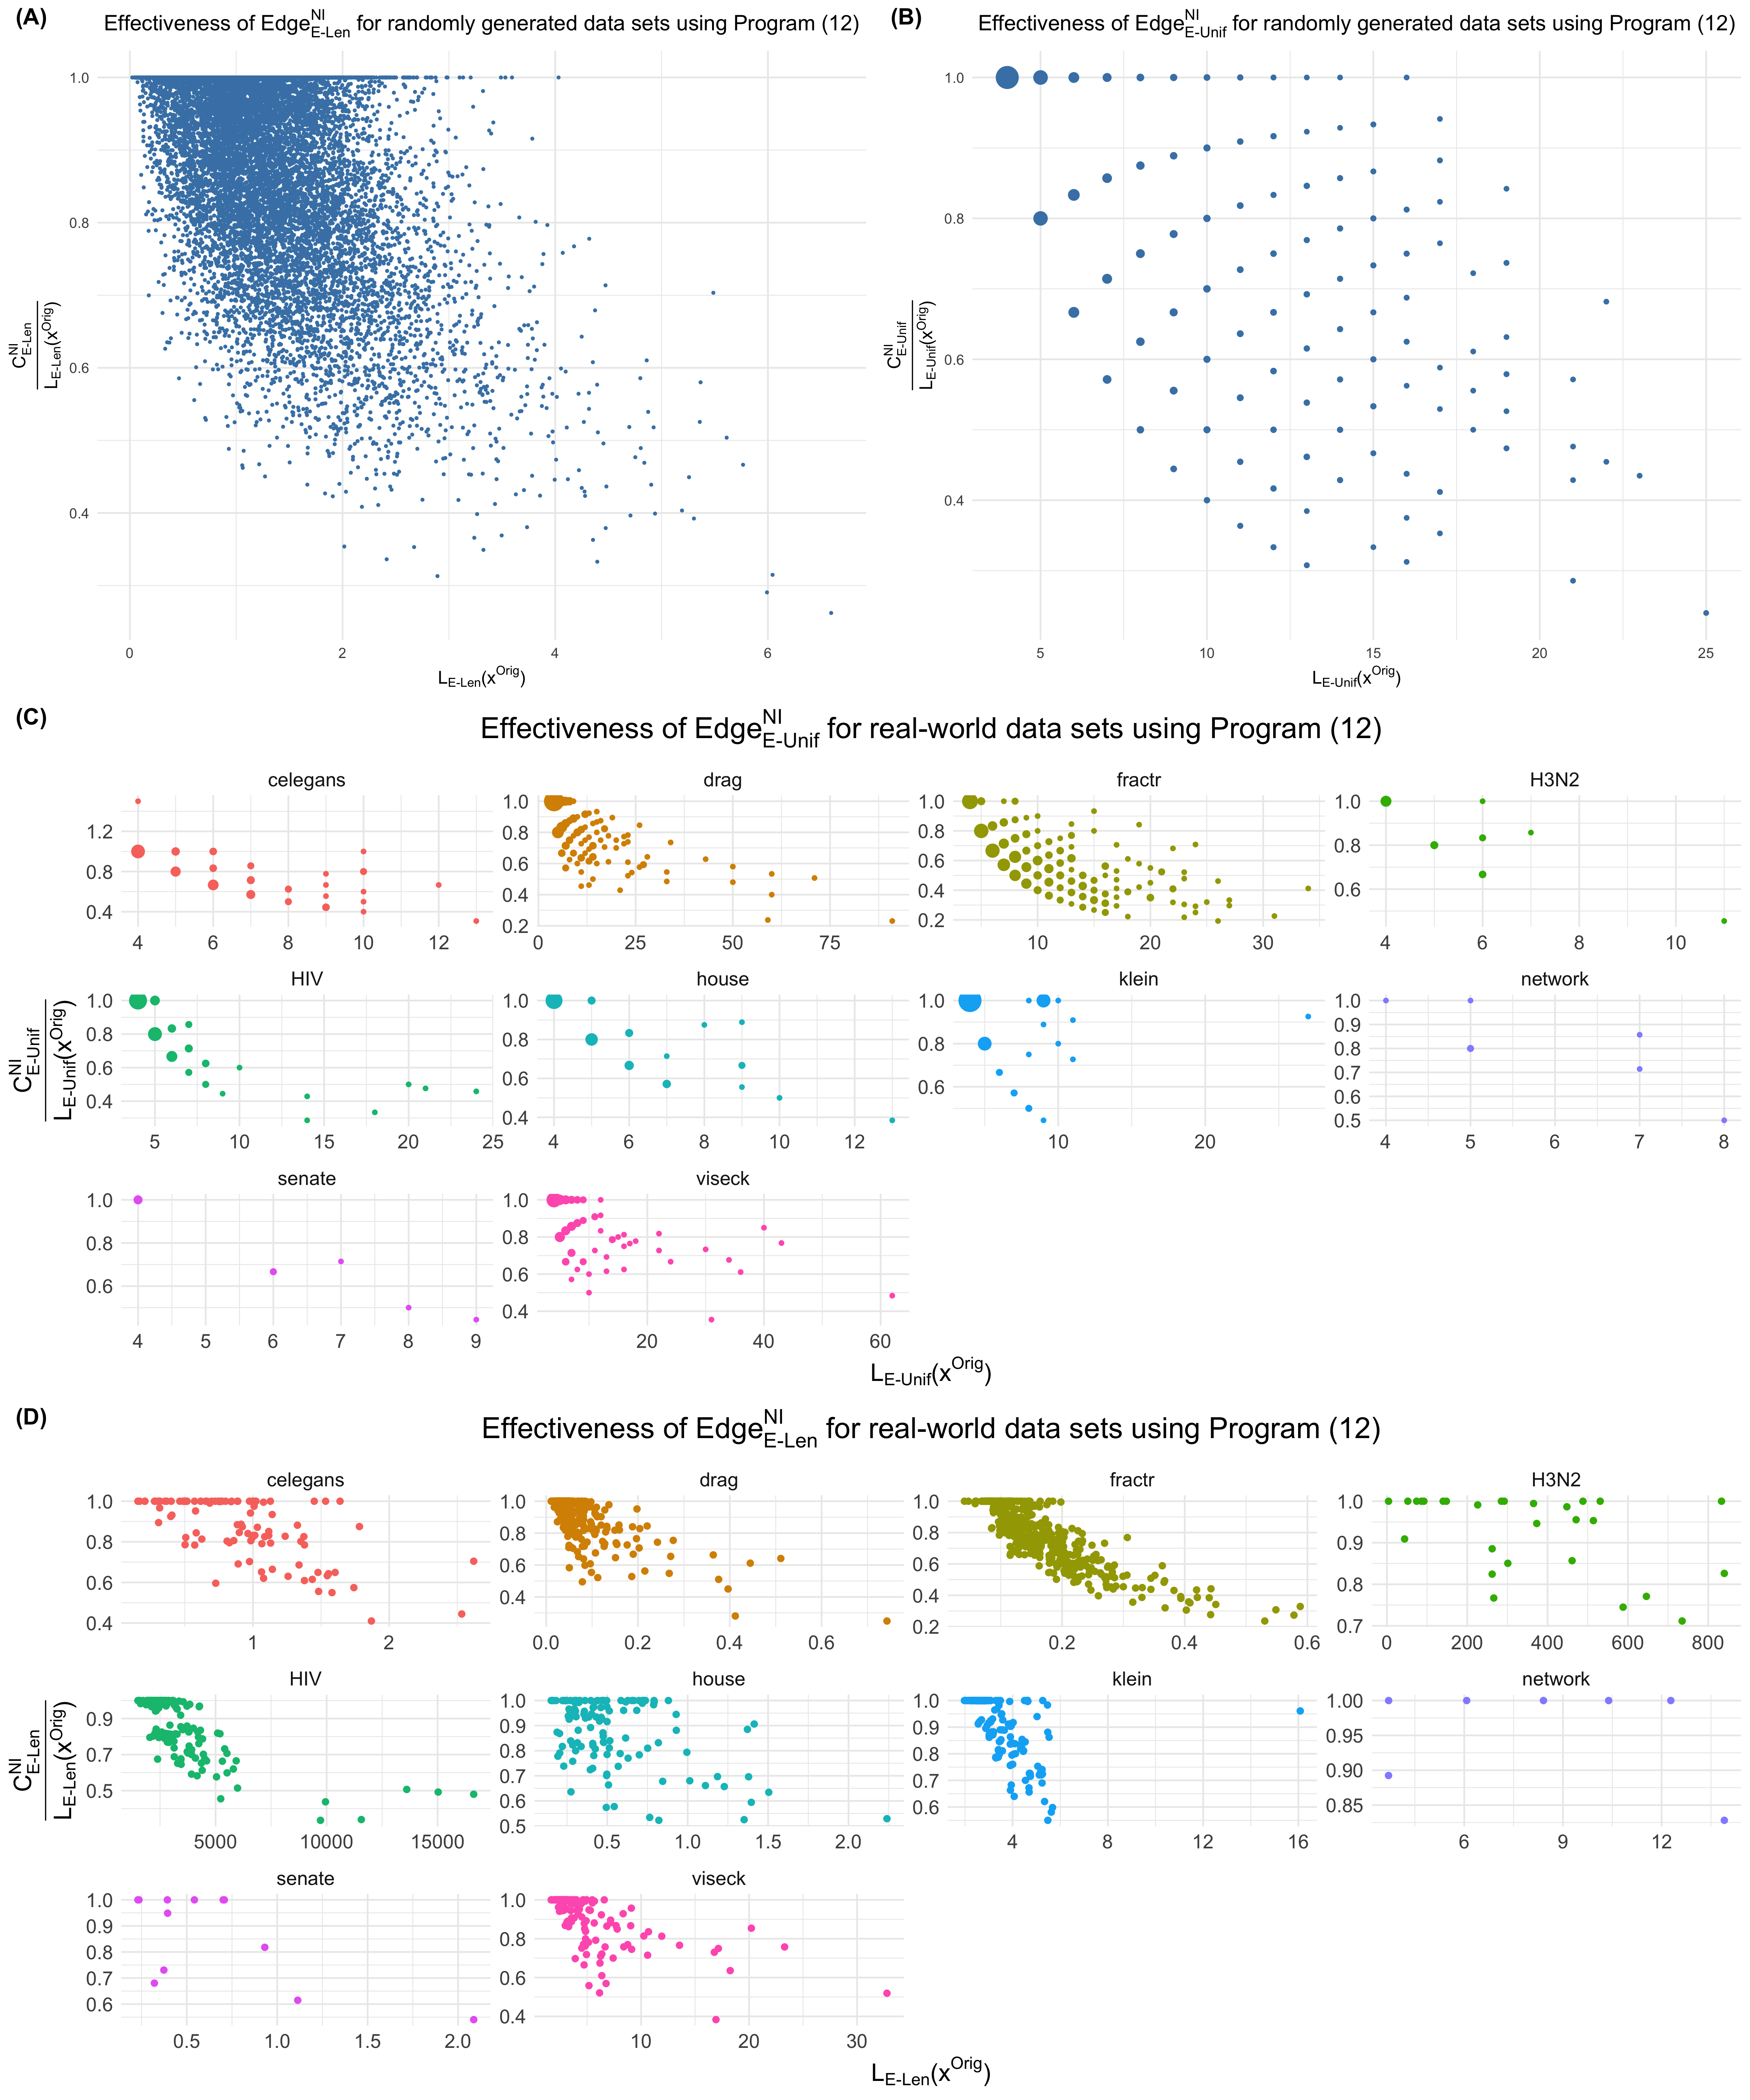
\includegraphics[width=0.95\textwidth]{figures/four_eff_df2.png}% This is a *.eps file
\end{center}
\caption{The effectiveness of length-weighted and uniform-weighted optimization for the randomly generated data sets and real-world data sets in reducing the size of the original cycle representative found by the persistence algorithm. In each subfigure, the horizontal axis is the size of the original representative and the vertical axis is the ratio between the size of the optimal representative and the size of the original representative. The uniform-weighted graphs appear more sparse because reductions in the cost $L_{T\text{-}Unif}(\originalrep)$ can only come in multiples of the reciprocal of the original length. The node size in the uniform-weighed graphs corresponds to the number of overlapping points. %\LL{updated! 0314}
}\label{fig:effectivenessall}
\end{figure}
% \end{landscape}

% \begin{figure}[h!]
% \begin{center}
% 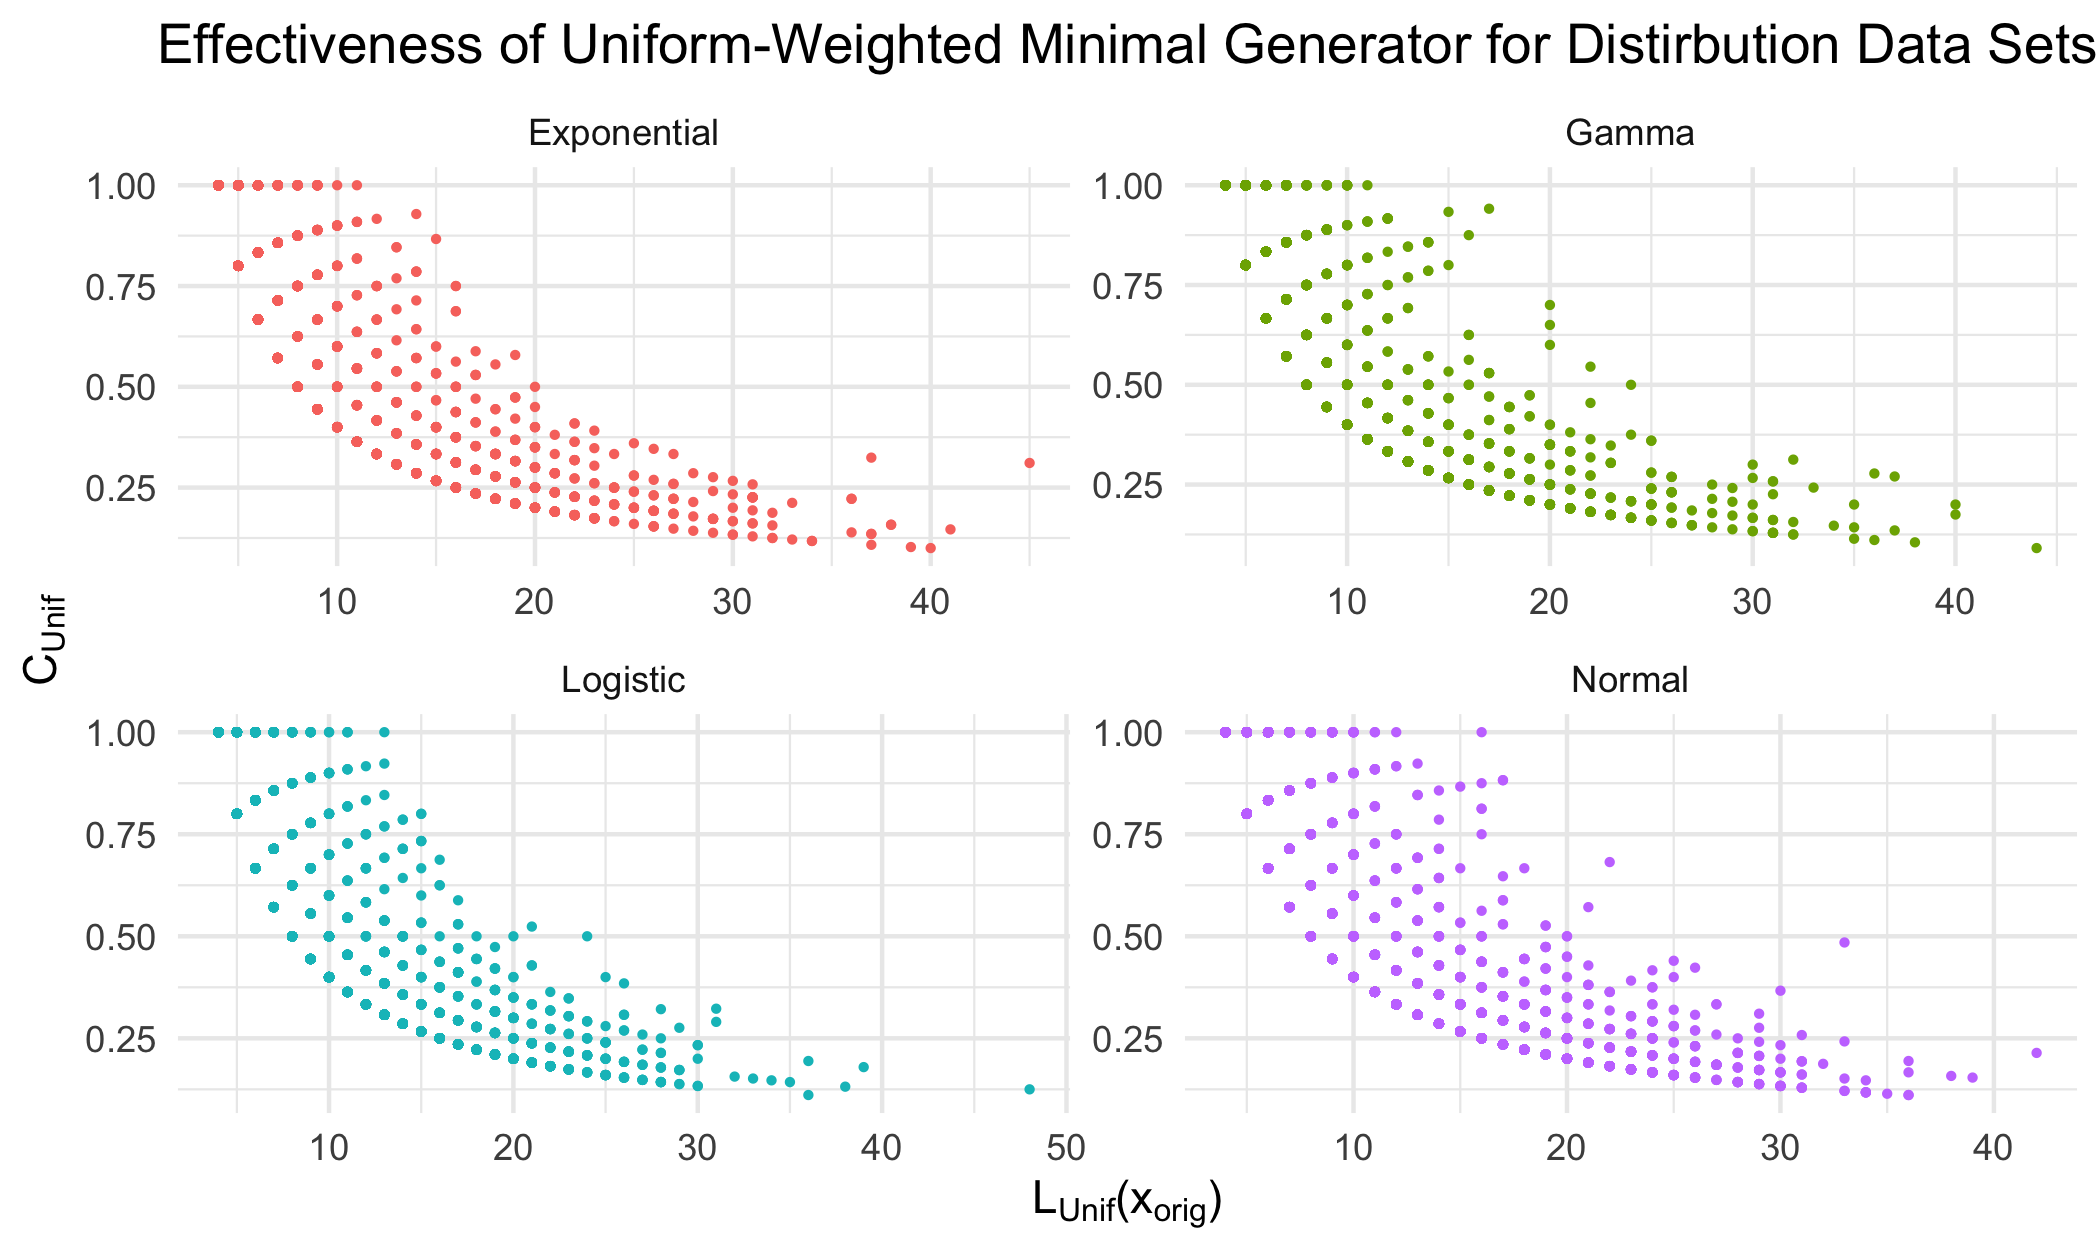
\includegraphics[width=1\textwidth]{figures/edge_eff_dist.png}% This is a *.eps file
% \end{center}
% \caption{Effectiveness of Uniform-Weighted Minimal Generator for Distribution Data Sets}\label{fig:edge_eff_dist}
% \end{figure}

% \begin{figure}[h!]
% \begin{center}
% 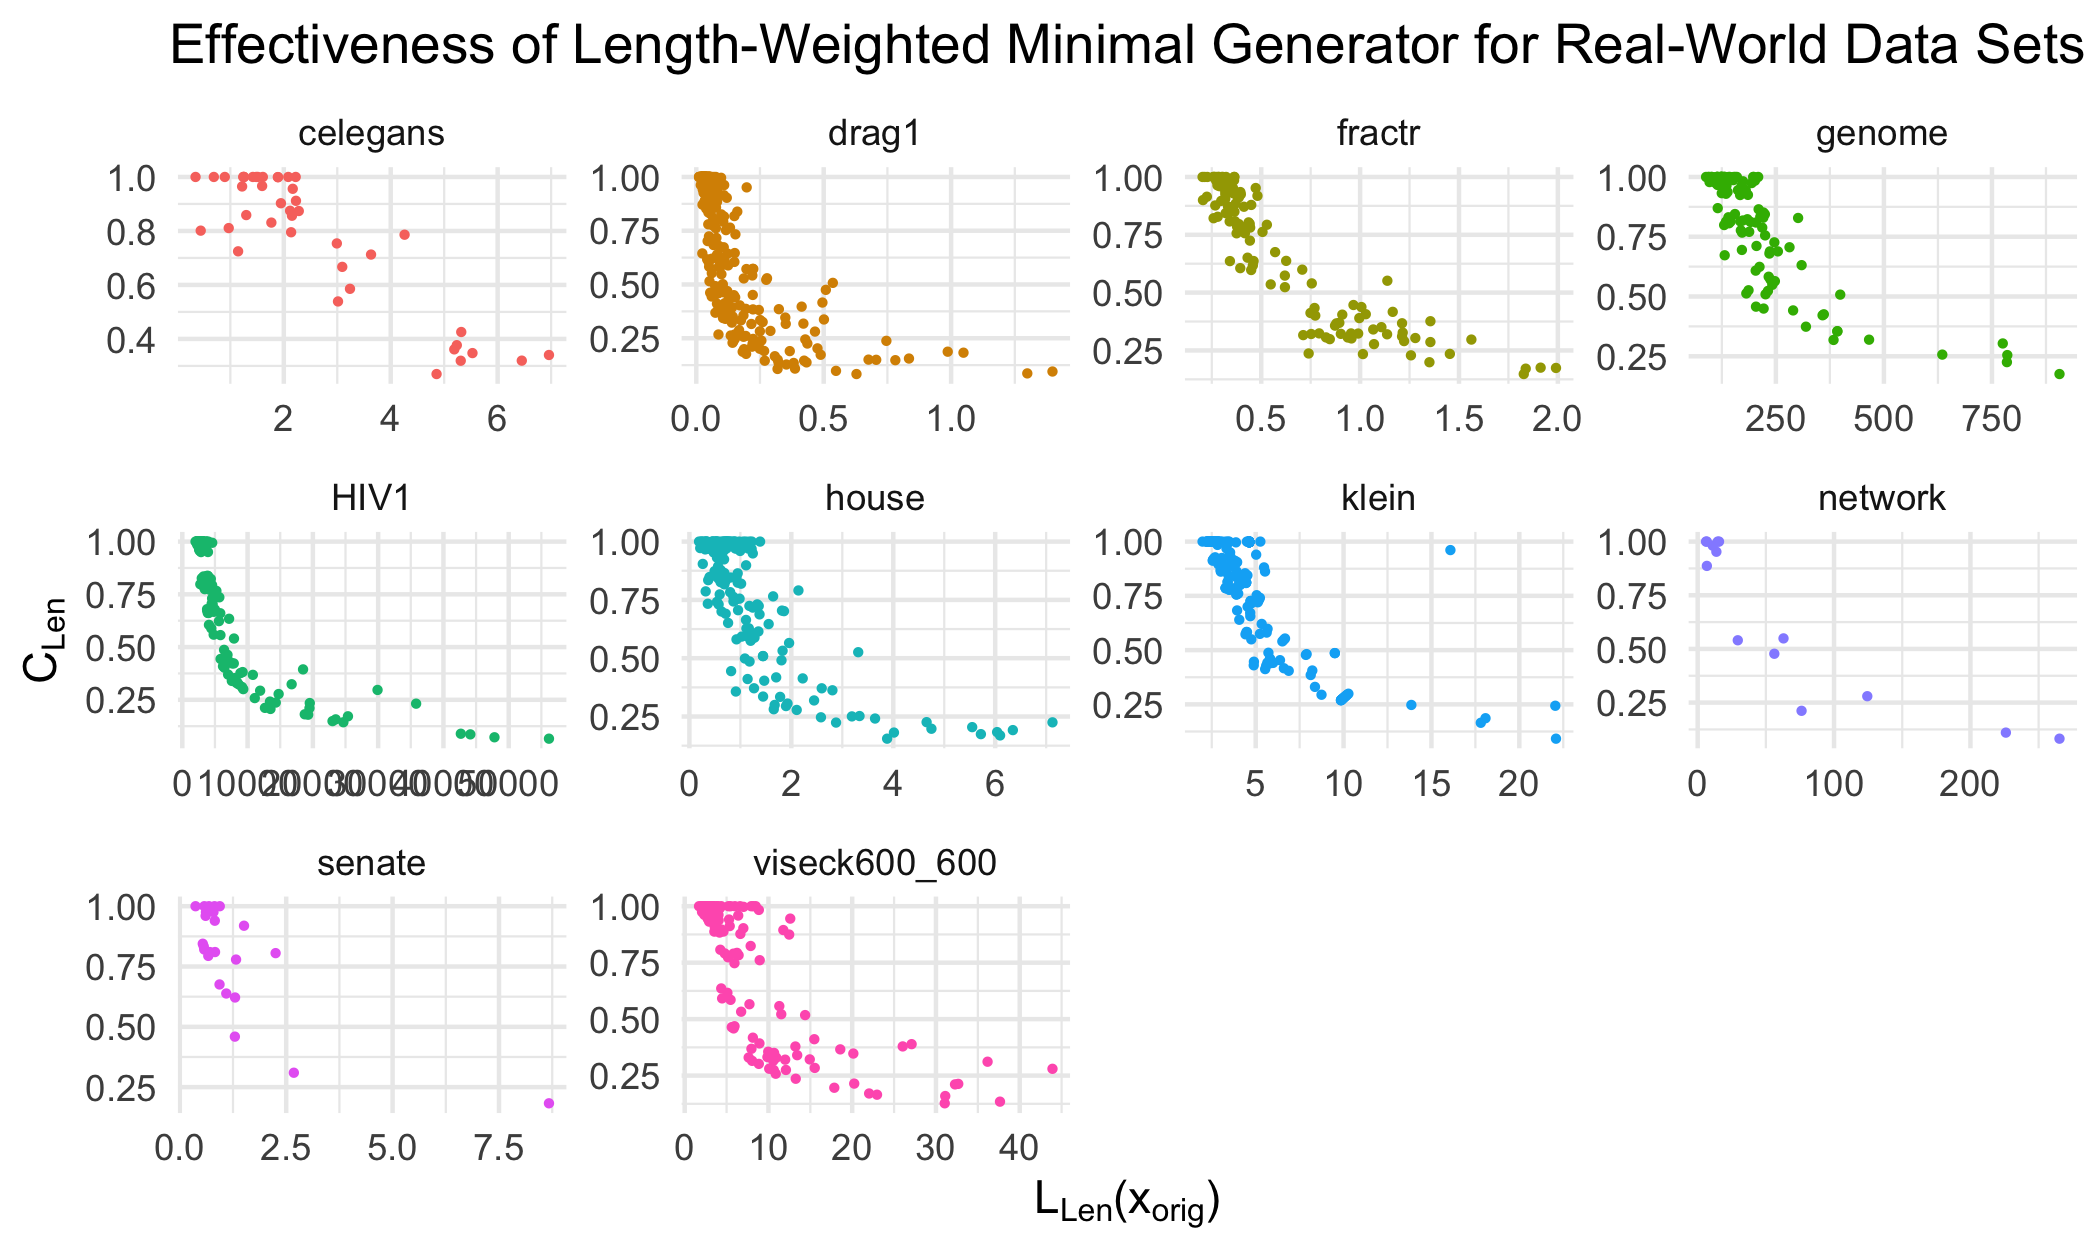
\includegraphics[width=1\textwidth]{figures/length_eff_df.png}% This is a *.eps file
% \end{center}
% \caption{Effectiveness of Length-Weighted Minimal Generator for Real-World Data Sets}\label{fig:length_eff_df}
% \end{figure}
% \begin{figure}[h!]
% \begin{center}
% 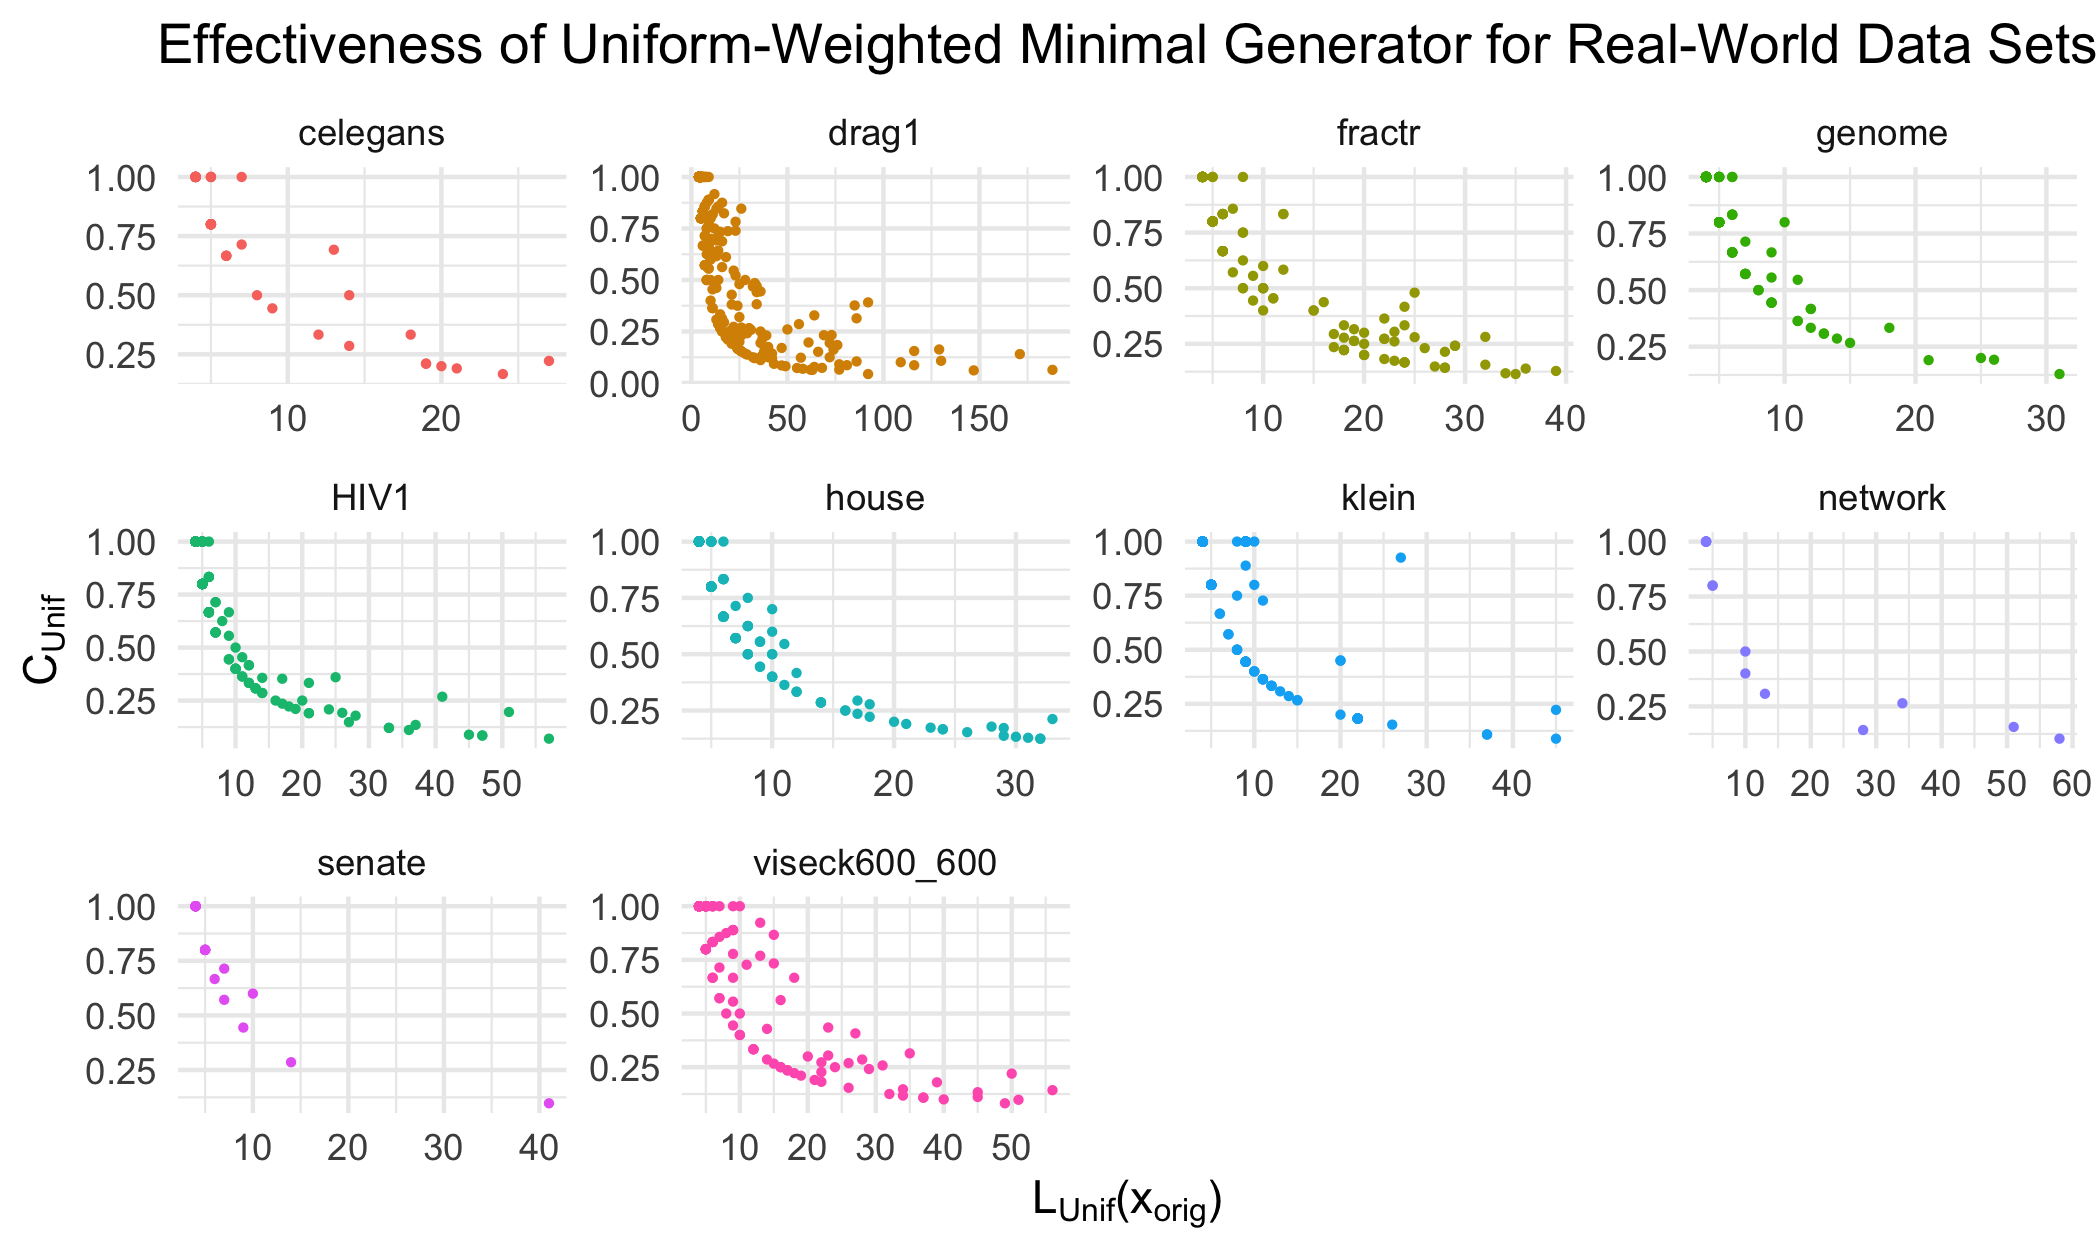
\includegraphics[width=1\textwidth]{figures/edge_eff_df.png}% This is a *.eps file
% \end{center}
% \caption{Effectiveness of Uniform-Weighted Minimal Generator for Real-World Data Sets}\label{fig:edge_eff_df}
% \end{figure}

\begin{figure}[h!]
\begin{center}
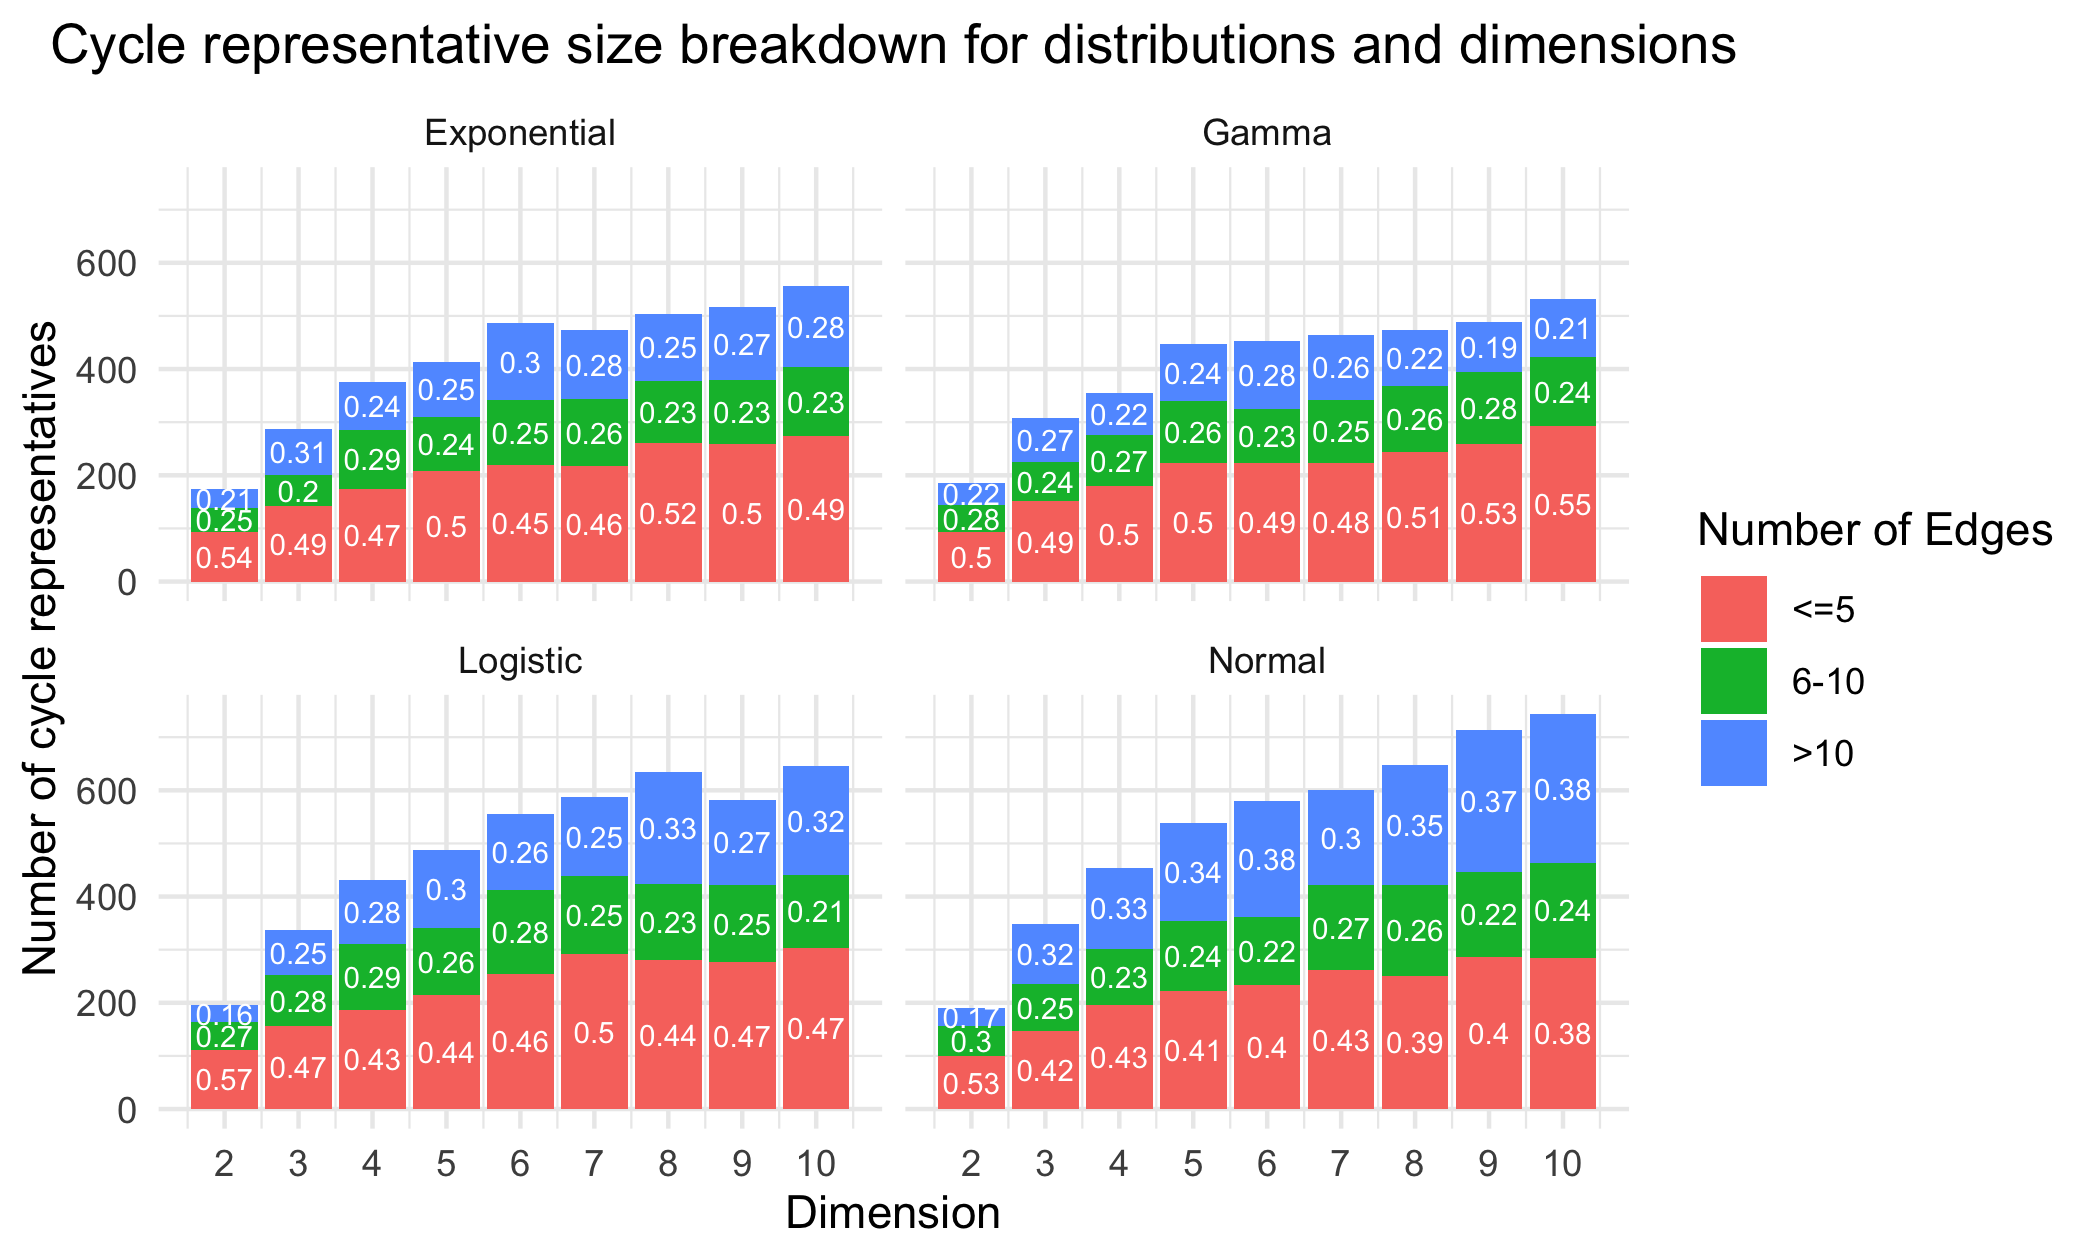
\includegraphics[width=1\textwidth]{figures/generator_breakdown.png}% This is a *.eps file
\end{center}
\caption{The number of original cycle representatives and the number of edges within each original representative for data described in \se \ref{sec: randompointclouds}. These plots aggregate all cycle representatives for each dimension of a particular distribution. The horizontal axis for each subplot is the dimension of the data set, and the vertical axis is the number of cycle representatives found in each dimension. In general, we see there are more cycle representatives in higher dimensional data sets. Each bar is partitioned by the number of edges of the representative. We observe that as dimension increases, there tend to be more cycle representatives with more edges. %\LL{updated 0314}
}\label{fig:gen_num_breakdown}
\end{figure}


% % \begin{figure}[h!]
% \begin{center}
% 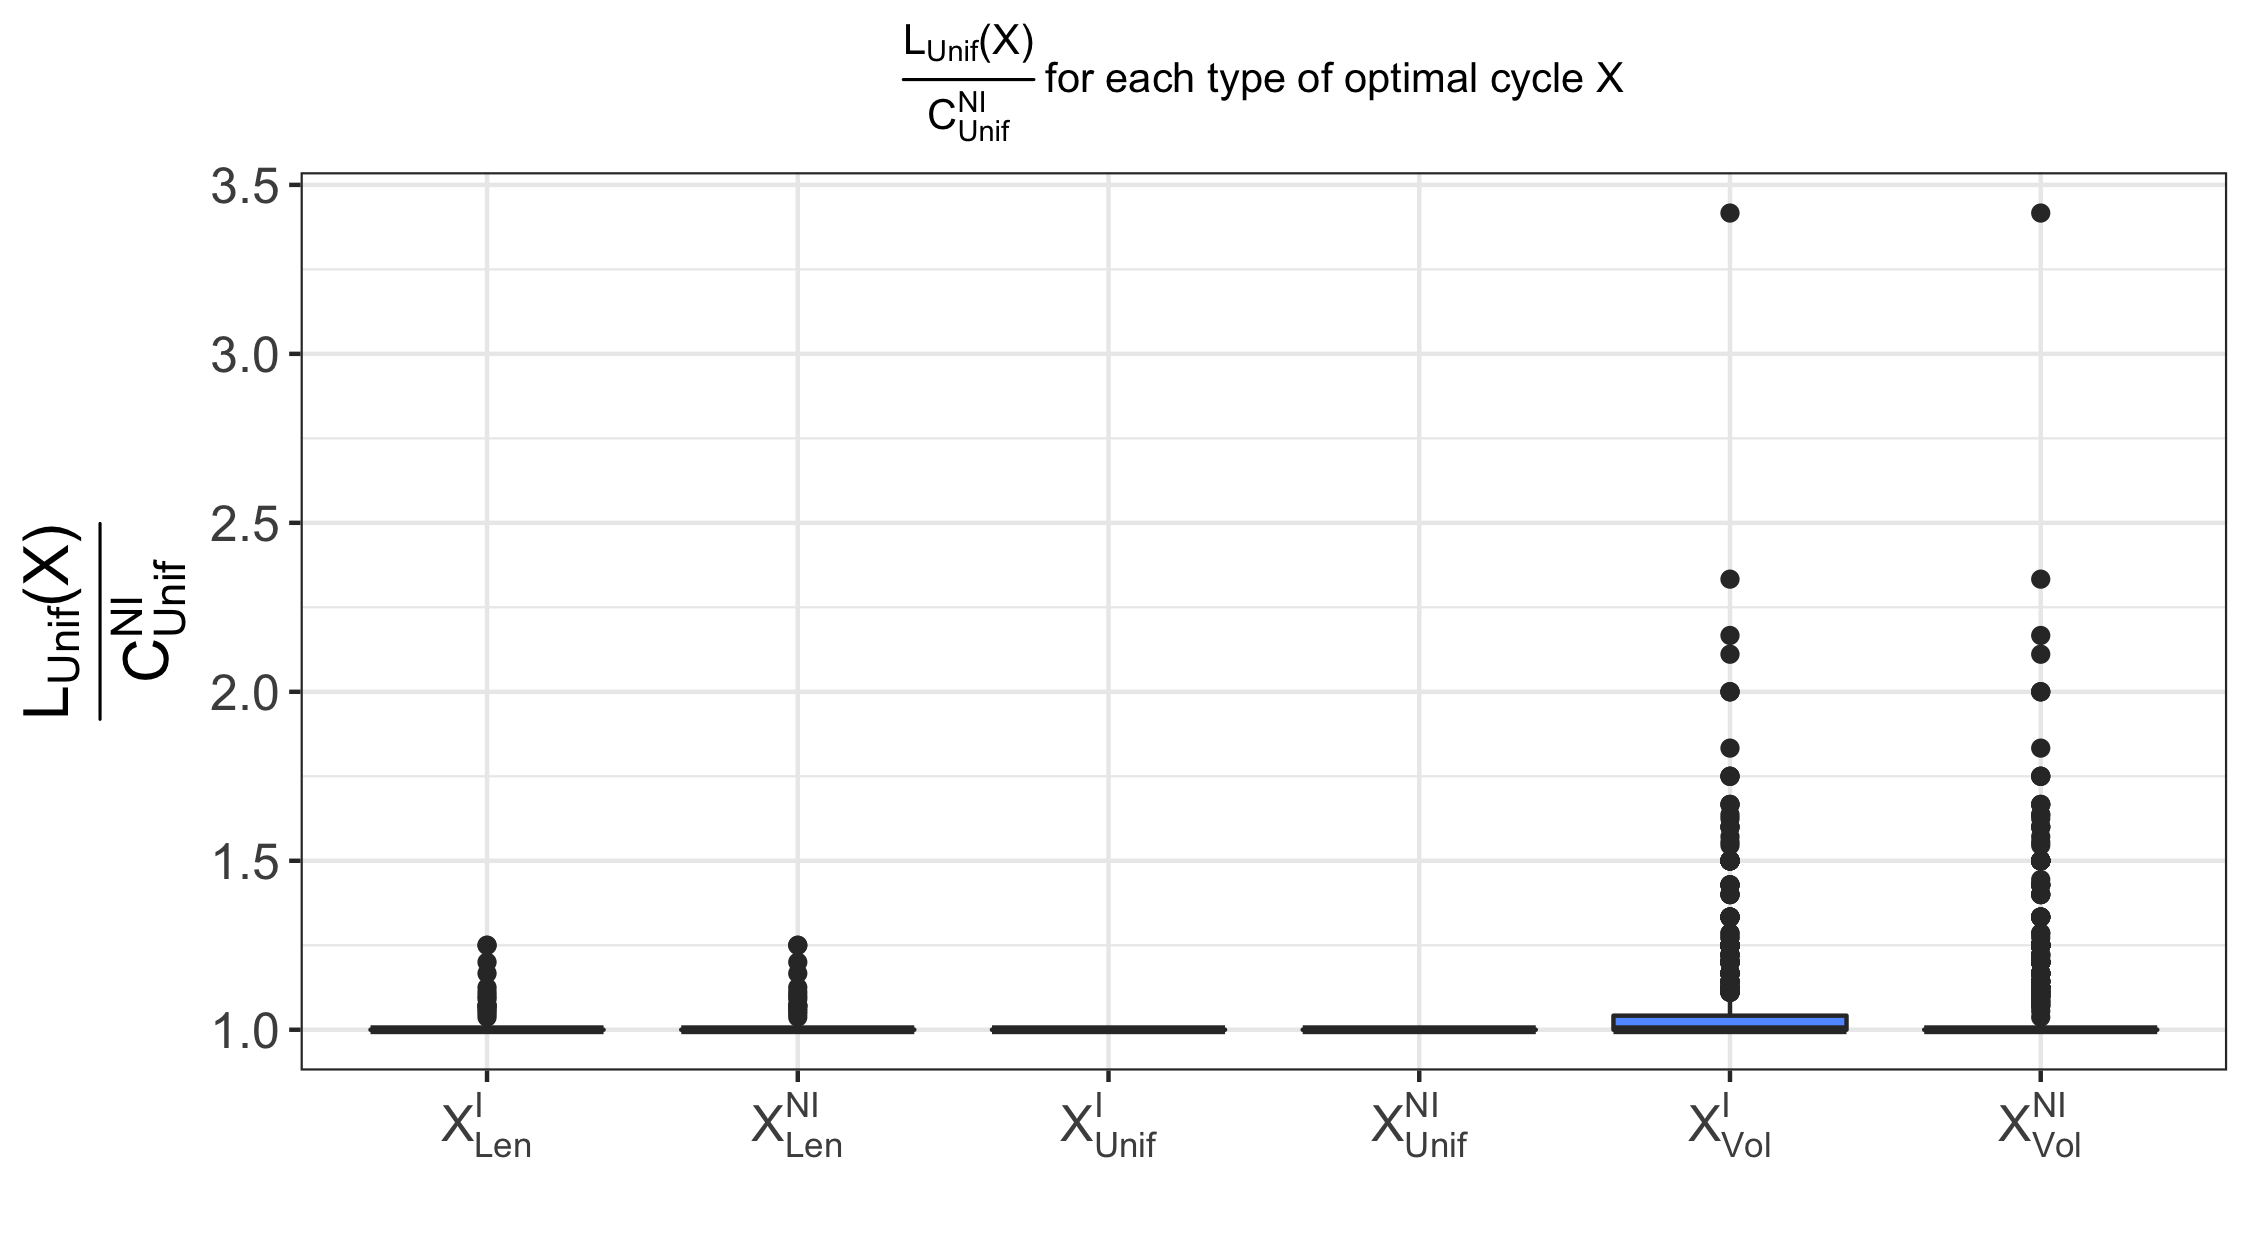
\includegraphics[width=\textwidth]{figures/edge_compare.png}
% \end{center}
% \caption{Box plots comparing the uniform-weighted loss of each type of optimal cycles against the uniform-weighted optimum cost. The $x$-axis is the type of optimal cycle and the $y$-axis is the ratio between the uniform-weighted cost of each type of optimal cycle and the actual uniform-weighted cost of the uniform-weighted minimal cycle (i.e. the number of edges in the cycle) without requiring integral solutions. We expect the middle two columns to be 1 as the optimums obtained whether requiring integral solutions or not are the same in all our experiments.}\label{fig:edgecompare}
% \end{figure}




% \begin{landscape}

\begin{table}[!h]
\caption{distmat}
    {\footnotesize{
    % \begin{tabular}{ |>{\centering\arraybackslash}m{3cm} | {\centering\arraybackslash}m{1.5cm} |  >{\centering\arraybackslash}m{1.8cm} | {\centering\arraybackslash}m{1.5cm} |  >{\centering\arraybackslash}m{2cm}|   >{\centering\arraybackslash}m{2cm}| >{\centering\arraybackslash}m{2cm} | >{\centering\arraybackslash}m{2cm}|  >{\centering\arraybackslash}m{2cm}| >{\centering\arraybackslash}m{1.3cm}| >{\centering\arraybackslash}m{2cm} | >{\centering\arraybackslash}m{2cm} |}
    
    \begin{tabular}{ |>{\centering}m{11em} *{11}{>{\centering\arraybackslash}m{4.5em} }|}
 \hline
  & \textbf{Klein} & \textbf{Vicsek}  & \textbf{C.elegans} & \textbf{HIV} & \textbf{Genome}  & \textbf{fractal R} & \textbf{network} & \textbf{house} & \textbf{senate} & \textbf{drag} & \textbf{H3N2}\\[0.5ex] 
 \hline 
 \hline
 \textbf{Ambient dimension} & 3 & 3 & 202 &  673 & 688 &  259 & 300 & 261 & 60 & 3 &  1,173\\   
 \textbf{\# points}   & 400 &  300  &  297 &   1088 &  1397  & 512 & 379 & 445  & 103 & 1,000 & 2,722\\ 
 \textbf{\# representatives}&   & 124  &  107 &174   &     & 438 & 7  & 126  & 12 &  & 28 \\  
 \textbf{$T$ persistence}   &   & 6.81 & 5.14 &728.51&     & 143.07 & 12.18  &  9.62 & 0.10 &  & 71,081.77  \\ 
 [0.5ex] 
\hline
\multicolumn{5}{c}{\textbf{\qquad Edge-loss persistent homological cycle representatives (\pr \eqref{eq:edgelossgeneral})}} &&&&&& \\
\hline
%  \textbf{Memory (GiB)}    & 5.56 & 3.05 & 199.52 & 181.27  & 7.71 & 72.17 & 7.16 & 0.15& 416.38\\ \hline        
 \textbf{$T\I_{E\text{-}Len}$ optimization} &   & 8.2 &  19.64&466.85  &     & 150.46 & 0.17 & 63.93  & 0.31 &  & 4,732.59	\\ 
 \textbf{$T\NI_{E\text{-}Len}$ optimization} &   & 6.61 &16.07  &403.63 &     & 86.95 & 0.13 & 48.65  & 0.22 &  & 4,540.55 \\ 
 \textbf{$T\I_{E\text{-}Unif}$ optimization} &   & 9.09 & 19.22 & 473.82 &     & 119.94 & 0.23 &  63.34 & 0.33 &  & 4,714.90	\\ 
  \textbf{$T\NI_{E\text{-}Unif}$ optimization} &   & 5.55 & 15.63 & 404.95 &     & 83.40 & 0.12 & 48.88  & 0.22 &  & 4,547.37 \\
  [0.5ex] 
\hline
\multicolumn{5}{c}{\textbf{Edge-loss filtered homological cycle represnetatives (\pr \eqref{eq:escolarargmin})}} &&&&&& \\
\hline
%  \textbf{Memory (GiB)}    & 5.56 & 3.05 & 199.52 & 181.27  & 7.71 & 72.17 & 7.16 & 0.15& 416.38\\ \hline        
 \textbf{$T\I_{E\text{-}Len}$ optimization} &   &8.64  &20.41  & 468.22 &     &  155.08&  0.17 &  62.2  & 0.30 &  & 2,999.24	\\ 
 \textbf{$T\NI_{E\text{-}Len}$ optimization} &   & 5.51 &16.15  & 403.74 &     & 88.66 &0.13  &  48.24 & 0.22 &  & 2,829.12	\\ 
 \textbf{$T\I_{E\text{-}Unif}$ optimization} &   & 8.32 &19.76  & 476.84  &     &  142.4&  0.24  & 61.82  & 0.31 &  & 2,937.16	\\ 
  \textbf{$T\NI_{E\text{-}Unif}$ optimization} &   & 5.63 & 16.23 & 406.97 &     & 87.59 &  0.12 & 48.11  &0.22  &  & 2,833.06	 \\
  [0.5ex] 
\hline
\multicolumn{5}{c}{\textbf{Triangle-loss persistent homological cycle representatives (\pr \eqref{eq:trianglelossgeneral})\qquad}} &&&&&& \\
\hline
 \textbf{$T\I_{T\text{-}Unif}$ optimization} & & 23.07  &783.06  & 63,227.14 &  &  10,187.41   & 2.71 & 221.07  & 0.26  &  & 39,140.67 \\ 
 \textbf{$T\NI_{T\text{-}Unif}$ optimization} & & 18.81 & 610.20 &60,459.49 &  &   8,441.76  & 2.08 & 170.95  & 0.23  &  & 36,401.50  \\ 
 \textbf{$T$ build all}  & & 0.88  &  &  &  & 45.28 & 0.05 &  4.85 & 0.03  &  & \\ 
\textbf{Total $T$ build part}  & & 3.06  &24.21 & 860.91 &  & 193.99 & 0.26 & 31.37  & 0.03  &  & 922.50 \\ \hline 
\end{tabular}
}%\LL{Updated 03/14}
}
\label{tab:realworldata}
\end{table}
% \end{landscape}
% \begin{table}[!h]
%     \centering
%     \begin{tabular}{ |c || c |c |c |c | c| c|c|c|c|c|}
%  \hline
%  & Klein & Vicsek600  & eleg & HIV & Genome  & fractal R & network & house & senate & drag\\[0.5ex] 
%  \hline 
%  Ambient dimension & 3 & 3    & 202 &  673 & 688 &  259 & 300 & 261 & 60 & 3\\\hline  
%  \# points &  400 &  300  &  297 &   1088 &  1397  & 512 & 379 & 445  & 103 & 1000\\\hline  
%  $T$ persistence &   95.56  & 8.74  & 3.39 & 552.80 &  1079.96  & 62.99 & 31.73 & 7.79 & 0.12 & 1037.70 \\ \hline
%  Memory (GiB) &   50.77  & 5.56 & 3.05 & 199.52 & 181.27  & 7.71 & 72.17 & 7.16 & 0.15& 416.38\\ \hline        
%  \# generators & 257 & 124  &42& 199& 117& 126&  13 & 133 & 19& 311\\ \hline
%  $T\I_{Len}$ optimization &2,253.14   & 358.72    & 47.75 &  8,140.87  & 48,109.66  & 2,700.03 &   17.05 & 347.09 &    1.18 & 8,305.27 \\ \hline
%  $T\NI_{Len}$ optimization& 2,163.14  & 308.56  & 26.53 & 5,101.00 &23,264.60  &2,000.97  &  11.43   &138.36   &  0.91  &7,280.97 \\ \hline 
%  $T\I_{Unif}$ optimization &2,323.93&   362.77&    47.62  &8,700.25& 46,754.56  &2,830.24  &  18.59   &311.09&     1.16&  8,339.93 \\ \hline
%   $T\NI_{Unif}$ optimization &2,212.52   &309.72  &  26.55  &5,004.96& 23,323.30&  2,222.38 &   11.54  & 138.73 &    0.90 &  7,305.24 \\ 
%  \hline
%  $T\I_{Vol}$ optimization &  & 140.04  &  223.97 &  16,691.24  & 16,328.65 &  6,849.59 &    7.52  & 204.31 &   0.36  &  443.89\\ \hline
%  $T\NI_{Vol}$ optimization&   & 130.95 & 169.08 & 14,547.61 & 14570.72 & 5,939.54&  8.01  & 172.66  &  0.30 & 398.79\\ \hline 
%  T build all triangles &   & 14.86 & 9.76 &  & - & 47.8 & 11.76  &   &  0.04 & 172.60\\ \hline 
% Total deleting time &   & 0.01 & 0.05 &  & &  & 0.00  &    &  0.00 & \\ \hline 
% Total build-part time &   &  &   8.28 &  475.37 & 437.75 & 268.57 &  1.06 & 28.42 &    & 242.14\\ \hline 

% \end{tabular}
% \caption{External Data Sets (Time measured in seconds)}
% \label{tab:data}
% \end{table}
% \end{center}




\begin{table}[!h]
\caption{\caption{Summary of the experimental results of the data sets from \cite{roadmap2017} as described in \se \ref{sec: realworlddata}. The rows include the ambient dimension, number of points, the number of cycle representatives in $\Homologies_1$, and the time (measured in seconds) it took to compute persistent homology for each data set. We also include the computation time taken to optimize the set of cycle representatives under six different optimization problems, and computation time of two different implementation choices for the triangle-loss optimal cycles: building the full $\partial_2$ boundary matrix once and extracting the part needed, or constructing part of the $\partial_2$ boundary matrix for each cycle representative. In this table, $T$ stands for computation time measured in seconds with subscripts indicating the type of the optimal cycle and superscripts indicating whether the program was solved using linear programming (NI) or integer programming (I). The time taken to construct the input to the optimization problem is included in the optimization time for edge-loss minimal cycle representatives, but is excluded and separately listed in the last two rows for the triangle-loss minimal cycle representatives. For triangle-loss cycles, we were able to compute $115$ out of the $117$ cycle representatives for the \textbf{Genome} data set and $52$ out of $57$ cycle representatives for the \textbf{H3N2} data set due to memory constraints. The numbers in the parenthesis represent the other optimization statistics corresponding to the triangle-loss optimal cycles we were actually able to compute. The last two rows compare two ways of building the input $\partial_2[:,\hat {\mathcal{F}}_{2}]$ matrix to the triangle-loss optimal cycle program. The penultimate row records the time of building the entire $\partial_{2}$ matrix once and then extracting columns born in the interval $\closedinterval$ for each representative. The last row records the total time to iteratively build the part of the boundary matrix $\partial_2[:,\hat {\mathcal{F}}_{2}]$ for each cycle representative.}
}
    {\footnotesize{
    % \begin{tabular}{ |>{\centering\arraybackslash}m{3cm} | {\centering\arraybackslash}m{1.5cm} |  >{\centering\arraybackslash}m{1.8cm} | {\centering\arraybackslash}m{1.5cm} |  >{\centering\arraybackslash}m{2cm}|   >{\centering\arraybackslash}m{2cm}| >{\centering\arraybackslash}m{2cm} | >{\centering\arraybackslash}m{2cm}|  >{\centering\arraybackslash}m{2cm}| >{\centering\arraybackslash}m{1.3cm}| >{\centering\arraybackslash}m{2cm} | >{\centering\arraybackslash}m{2cm} |}
    
    \begin{tabular}{ |>{\centering}m{11em} *{11}{>{\centering\arraybackslash}m{4.5em} }|}
 \hline
  & \textbf{Klein} & \textbf{Vicsek}  & \textbf{C.elegans} & \textbf{HIV} & \textbf{Genome}  & \textbf{fractal R} & \textbf{network} & \textbf{house} & \textbf{senate} & \textbf{drag} & \textbf{H3N2}\\[0.5ex] 
 \hline 
 \hline
 \textbf{Ambient dimension} & 3 & 3    & 202 &  673 & 688 &  259 & 300 & 261 & 60 & 3 &  1,173\\   
 \textbf{\# points}   & 400 &  300  &  297 &   1088 &  1397  & 512 & 379 & 445  & 103 & 1,000 & 2,722\\ 
 \textbf{\# representatives} & 257 & 124  &42& 199& 117 (115) & 126&  13 & 133 & 19& 311 & 57 (53) \\  
 \textbf{$T$ persistence} &   66.21  & 5.48  & 3.41 & 552.80 &  967.61  & 62.99 & 10.23 & 7.79 & 0.12 & 948.16 & 23,362.05 \\ 
 [0.5ex] 
\hline
\multicolumn{5}{c}{\textbf{\qquad Edge-loss persistent homological cycle representatives (\pr \eqref{eq:edgelossgeneral})}} &&&&&& \\
\hline
%  \textbf{Memory (GiB)}    & 5.56 & 3.05 & 199.52 & 181.27  & 7.71 & 72.17 & 7.16 & 0.15& 416.38\\ \hline        
 \textbf{$T\I_{E\text{-}Len}$ optimization} & 16.01 & 8.24 & 13.22 & 957.48 & 656.05 & 78.1 & 0.72 & 66.23 & 0.38 & 45.14 &5469.85	\\ 
 \textbf{$T\NI_{E\text{-}Len}$ optimization} & 11.28 & 5.66 & 9.94 & 850.09 & 491.69 & 53.85 & 0.57 & 48.53 & 0.29 & 34.73 &4989.13	\\ 
 \textbf{$T\I_{E\text{-}Unif}$ optimization} & 14.59 & 8.66 & 13.36 & 980.82 & 689.51 & 82.17 & 0.76 & 66.67 & 0.4 & 45.51 & 5274.77	\\ 
  \textbf{$T\NI_{E\text{-}Unif}$ optimization} & 11.38 & 5.66 & 10.39 & 872.12 & 492.66 & 54.96 & 0.56 & 49.72 & 0.31 & 33.88 & 4991.39	\\
  [0.5ex] 
\hline
\multicolumn{5}{c}{\textbf{Edge-loss filtered homological cycle represnetatives (\pr \eqref{eq:escolarargmin})}} &&&&&& \\
\hline
%  \textbf{Memory (GiB)}    & 5.56 & 3.05 & 199.52 & 181.27  & 7.71 & 72.17 & 7.16 & 0.15& 416.38\\ \hline        
 \textbf{$T\I_{E\text{-}Len}$ optimization} & 16.93 & 8.05 & 13.88 & 557.47 & 1144.17 & 75.56 & 0.97 & 61.84 & 0.35 & 67.77 & 5464.05	\\ 
 \textbf{$T\NI_{E\text{-}Len}$ optimization} & 10.29 & 6.15 & 11.3 & 464.34 & 973.15 & 53.86 & 0.66 & 43.22 & 0.26 & 50.25 & 4992.40	\\ 
 \textbf{$T\I_{E\text{-}Unif}$ optimization} & 15.14 & 8.53 & 13.2 & 562.57 & 1191.44 & 79.31 & 0.68 & 61.42 & 0.35 & 68.63 & 5277.85	\\ 
  \textbf{$T\NI_{E\text{-}Unif}$ optimization} & 11.07 & 5.94 & 10.35 & 467.22 & 981.72 & 53.86 & 0.53 & 43.66 & 0.43 & 54.05 &4988.87	 \\
  [0.5ex] 
\hline
\multicolumn{5}{c}{\textbf{Triangle-loss persistent homological cycle representatives (\pr \eqref{eq:trianglelossgeneral})\qquad}} &&&&&& \\
\hline
 \textbf{$T\I_{T\text{-}Unif}$ optimization} &   185.92 &72.69 &  477.53 &  21,072.34  & 16,379.86&  5,300.92 &     25.33  & 421.45 &    0.91 &  384.91 & 12,341.58\\ 
 \textbf{$T\NI_{T\text{-}Unif}$ optimization} & 103.26 & 62.42 & 372.46 & 18,958.53 & 14,535.42 & 4,411.80& 20.86  & 342.05 & 0.79 & 277.93 & 11,467.15\\ 
 \textbf{$T$ build all}  &5.52 & 3.56 &10.07 &  826.25& - & 47.8 & 12.55  & 6.82  &  0.08 & 172.60 & -\\ 
% Total deleting time   & 0.01 & 0.05 &  & &  & 0.00  &    &  0.00 & \\ \hline 
\textbf{Total $T$ build part} & 6.13  & 3.30 &   8.28 &  451.41 &415.79& 94.86 & 0.87 & 33.40 &  0.06  & 198.27 & 895.36\\ \hline 
\end{tabular}
}%\LL{Updated 03/14}
}
\label{tab:realworldata}
\end{table}

\setlength{\tabcolsep}{10pt}

\renewcommand{\arraystretch}{1.5}
\begin{table}[!h]
\caption{Summary of the experimental results for the synthetic, randomly generated data sets described in \se \ref{sec: randompointclouds}. For each distribution, we sample $10$ data sets each containing $100$ points in ambient dimensions from $2$-$10$. The computation time in this table averages the $10$ random samples for each dimension and distribution combination. The number of cycle representatives is totaled over the $90$ samples for each distribution. The rows of this table are analogous to those of \tab \ref{tab:realworldata}, excluding the penultimate row of that table, as the time comparison is only done for the large real-world data sets.} 
\footnotesize
    \centering
    \begin{tabular}{ |c || c |c |c |c |}
 \hline
 & \textbf{Normal} & \textbf{Gamma}  & \textbf{Logistic} & \textbf{Exponential}  \\[0.5ex] 
 \hline 
 \hline
 \textbf{Ambient dimension} & 2-10 & 2-10    & 2-10 &  2-10  \\\hline  
 \textbf{Average \# points} &  100 &  100  &  100 &   100  \\\hline  
  \textbf{Total \# representatives} & 4815 & 3706  & 4456 & 3788 \\ \hline
 \textbf{Average $T$ persistence (seconds)} &   2.80  & 2.12    & 2.01 & 2.63 \\
%  Memory (GiB) &   116.16  & 85.23  & 79.24 & 199.52  \\ \hline 
[0.5ex] 
\hline
\multicolumn{1}{c}{\textbf{Edge-loss persistent homological cycle representatives (\pr \eqref{eq:edgelossgeneral})}} && \\
\hline
 \textbf{Average total $T\I_{E\text{-}Len}$ optimization} &5.52 & 6.01 & 5.65 & 5.91 \\ \hline
 \textbf{Average total $T\NI_{E\text{-}Len}$ optimization} &  4.37 & 4.55 & 4.32 & 4.47 \\ \hline 
 \textbf{Average total $T\I_{E\text{-}Unif}$ optimization} & 5.31 & 5.97 & 5.45 & 5.90 \\ \hline
 \textbf{Average total $T\NI_{E\text{-}Unif}$ optimization} & 4.08 & 4.58 & 4.23 & 4.51 \\ 
 [0.5ex] 
\hline
\multicolumn{1}{c}{\textbf{Edge-loss filtered homological cycle representatives (\pr \eqref{eq:escolarargmin})}} && \\
\hline
 \textbf{Average total $T\I_{E\text{-}Len}$ optimization} &5.32 & 6.46 & 6.27 & 6.88 \\ \hline
 \textbf{Average total $T\NI_{E\text{-}Len}$ optimization} & 4.07 & 5.05 & 4.78 &5.11 \\ \hline 
 \textbf{Average total $T\I_{E\text{-}Unif}$ optimization} &5.23 & 6.46 & 6.25 & 6.66\\ \hline
 \textbf{Average total $T\NI_{E\text{-}Unif}$ optimization} & 4.17 & 4.94 & 4.61 & 5.29\\ 
[0.5ex] 
\hline
\multicolumn{1}{c}{\textbf{Triangle-loss persistent homological cycle representatives (\pr \eqref{eq:trianglelossgeneral})}} &&& \\
\hline
 \textbf{Average total $T\I_{T\text{-}Unif}$ optimization} &16.86 & 25.7 &17.55 & 26.30\\ 
 \hline
 \textbf{Average total $T\NI_{T\text{-}Unif}$ optimization} &  14.73 & 22.21 & 15.42 & 21.86 \\ 
 \hline
   \textbf{Average total $T$ build all} & 1.40 & 1.71 &  1.56 & 1.07 \\ 
  \hline
  \textbf{Average total $T$ build part } & 3.51 & 1.54 &    1.61 & 1.56 \\ 
 \hline
 
\end{tabular}
\label{tab:distributiondata} %\LL{updated 03/14}
\end{table}



\newcolumntype{L}{>{\centering\arraybackslash}m{3cm}}

% \setlength{\tabcolsep}{7pt}

\renewcommand{\arraystretch}{1.5}
\begin{table}[!h]
\centering
\caption{Computation time of three differently sized input boundary matrices to edge-loss and triangle-loss methods. The superscripts denote whether the program requires an integral solution or not, and the subscripts indicate the type of optimal cycle. All time is measured in seconds. We perform experiments on a small-sized data set (\textbf{Senate}) that consists of $103$ points in dimension $60$ and a medium-sized data set (\textbf{House}) that contains $445$ points in dimension $261$. For edge-loss methods, we consider three implementations to solve these optimization problems: using the full boundary matrix $\partial_2$, using the basis columns and all rows $\partial_2[:, \hat \goodtriangles]$, and using the basis columns and deleting rows corresponding to edges born after the birth time of the cycle $\partial_2[\goodedges, \hat \goodtriangles]$. For triangle-loss methods, we consider three approaches to solve these optimization problems: zeroing out the columns in the boundary matrix outside of $[b_i,d_i]$ denoted as $\partial_{2_{zero}}$, deleting columns outside of this range $\partial_2[:,\hat {\mathcal{F}}_{2}]$, and deleting both columns outside of $[b_i, d_i]$ and rows born after $d_i$ denoted $\goodvolmatrix$. The \textbf{House} data set was too large to implement the first method.}\label{unif-acceleration-table}
\footnotesize
\begin{tabular}{ |>{\centering}m{11em}   >{\centering\arraybackslash}m{8em}>{\centering\arraybackslash}m{8em}  >{\centering\arraybackslash}m{8em} >{\centering\arraybackslash} m{8em}|}
 \hline
 & \multicolumn{4}{c|}{\textbf{Edge-loss Optimal Cycles (\pr \eqref{eq:edgelossgeneral})}} \\
\cline{3-4}
  & \textbf{T}  & \textbf{$ \partial_2$}  & \textbf{$\partial_2[:, \hat \goodtriangles]$}  & \textbf{$\partial_2[\goodedges, \hat \goodtriangles]$}  \\  [0.5ex]  \hline \hline
    \multirow{4}{*}{\textbf{Small Data Set (Senate)}} & 
 $T_{E\text{-}Unif}\NI$ & 1.06& 1.03 &	0.41  \\  &
  $T_{E\text{-}Unif}\I$ &1.25 &1.23	& 0.60 \\  &
    $T_{E\text{-}Len}\NI$ &1.05&  1.05 &	0.41   \\   &
  $T_{E\text{-}Len}\I$  & 1.23 &1.19 & 0.65 \\ 
  \hline 
  \multirow{4}{*}{\textbf{Medium Data Set (House)}} & 
 $T_{E\text{-}Unif}\NI$ & 184.70 & 122.72 &	47.10  \\ &
  $T_{E\text{-}Unif}\I$ &188.88 & 147.27	&  64.64 \\  &
    $T_{E\text{-}Len}\NI$ &184.41&  121.80 &	46.02    \\   &
  $T_{E\text{-}Len}\I$ & 193.01 & 146.46 & 63.87 \\ [0.5ex] \hline \hline
   & \multicolumn{4}{c|}{\textbf{Triangle-loss Optimal Cycles (\pr \eqref{eq:trianglelossgeneral})}} \\ \cline{3-4}
  & \textbf{\textbf{T}}  & \textbf{$\partial_{2_{zero}}$}  & \textbf{$\partial_2[:,\hat {\mathcal{F}}_{2}]$}  & \textbf{$\goodvolmatrix$} \\[0.5ex] 
 \hline 
 \hline
 \multirow{2}{*}{\textbf{Small Data Set (Senate)}}& 
 $T_{T\text{-}Unif}\NI$    & 23.25   & 0.99  & 0.59 \\  &
  $T_{T\text{-}Unif}\I$   & 25.31  & 1.06   & 0.66   \\ \hline
  \multirow{2}{*}{\textbf{Medium Data Set (House)}} & 
 $T_{T\text{-}Unif}\NI$   
   &  -  &	286.10 &   194.70 \\ &
  $T_{T\text{-}Unif}\I$  
    & -	& 317.45  &  237.73\\\hline 
\end{tabular}


%\caption{Computation time of three differently sized input boundary matrices optimization to find volume optimal cycles when solving Equations \eqref{eq:LP-vol} and \eqref{eq:MIP-vol}. The superscripts denote whether the program requires an integral solution or not, and the subscripts indicate the type of optimal cycle. All time is measured in seconds. We perform experiments on a small-sized data set (\textbf{Senate}) that consists of $103$ points in dimension $60$ and a medium-sized data set (\textbf{House}) that contains $445$ points in dimension $261$.  We consider three approaches to solve these optimization problems: zeroing out the columns in the boundary matrix outside of $[b_i,d_i]$, deleting columns outside of this range, and deleting both columns outside of $[b_i, d_i]$ and rows born after $d_i$. We do not include the computation time for zeroing out for the medium data set because it was too large.}
\label{tab:implementationcompare}
\end{table}

%\setlength{\tabcolsep}{9pt}

\renewcommand{\arraystretch}{1.5}
\begin{center}
\begin{table}[]
\caption{{\normalsize{Classifying the coefficients of the optimal cycles for all of the real-world data discussed in Section 5.1 as well as all of the synthetic sets discussed in Section 5.2. The rows are labeled by the coefficient type of the cycle representatives: ``Integral'' means the coefficients for the cycle representative $\optimalrep$ are in $\mathbb{Z}$ and ``In $\{-1,0,1\}$'' means the coefficients for the representative $\optimalrep$ are in $\{-1,0,1\}$. For the columns, $\optimalrep$ represents the optimal representative with its superscript indicating the type of optimization problem: $I$ for integer programming and $NI$ for linear programming, and its subscript indicating the type of optimal cycle: ${E\text{-}Len}, E\text{-}Unif, T\text{-}Unif$ refer to edge loss length-weighted minimal (minimizing total length of $1$-simplices), edge loss uniform (minimizing total number of $1$-simplices), and triangle loss uniform (minimizing the number of $2$-simplices a cycle representative bounds), respectively.}}}
\centering

% \begin{tabular}{|p{2cm} ||p{0.6cm} p{0.6cm} p{0.6cm} p{0.6cm} p{0.6cm}|p{0.6cm}| |p{0.6cm}|p{0.6cm}|p{0.6cm}|p{0.6cm}|p{0.6cm}|p{0.6cm}|}

{\scriptsize{ \begin{tabular}{ |>{\centering}m{7em} *{10}{>{\centering\arraybackslash}m{2.5em} }|}
 \hline
 & \multicolumn{10}{c|}{\textbf{Edge-loss filtered homological optimal cycles} (Program \eqref{eq:edgelossgeneral})} \\
\hline
& \multicolumn{4}{c}{\textbf{Randomly Generated Data Sets}} & & 
 \multicolumn{4}{c}{\textbf{Real-World Data Sets}} &  \\  \cline{2-5}  \cline{7-10}

\textbf{Coefficient Type} & $\x\I_{E\text{-}Len}$ & $\x\NI_{E\text{-}Len}$ & $\x\I_{T\text{-}Unif}$ & $\x\NI_{E\text{-}Unif}$ &  & $\x\I_{E\text{-}Len}$ & $\x\NI_{E\text{-}Len}$ & $\x\I_{E\text{-}Unif}$ & $\x\NI_{E\text{-}Unif}$ & \\
\hline
\textbf{Integral}  & $100\%$ &$100\%$&   $100\%$ & $100\%$ &  & $100\%$ &$100\%$&  $100\%$ & $100\%$ & \\
\textbf{In $\{-1, 0, 1\}$} &  $100\%$  & $100\%$   &$100\%$ & $100\%$ & & $100\%$ &$100\%$&  $100\%$ & $100\%$ & \\ \hline
 & \multicolumn{10}{c|}{\textbf{Edge-loss persistent homological optimal cycles} (\pr (8))}  \\\hline

& \multicolumn{4}{c}{\textbf{Randomly Generated Data Sets}} & & 
 \multicolumn{4}{c}{\textbf{Real-World Data Sets}} &  \\  \cline{2-5}  \cline{7-10}
 \textbf{Coefficient Type} & $\x\I_{E\text{-}Len}$ & $\x\NI_{E\text{-}Len}$ & $\x\I_{T\text{-}Unif}$ & $\x\NI_{E\text{-}Unif}$ &  & $\x\I_{E\text{-}Len}$ & $\x\NI_{E\text{-}Len}$ & $\x\I_{E\text{-}Unif}$ & $\x\NI_{E\text{-}Unif}$ & \\

\hline 
\textbf{Integral}  & $100\%$ &$100\%$&   $100\%$ & $100\%$  &&  $100\%$ & $100\%$ &  $100\%$ & $99.94\%$ & \\
\textbf{In $\{-1, 0, 1\}$} &  $100\%$  & $100\%$   &$100\%$ & $100\%$ &  & $100\%$ & $100\%$&  $100\%$ & $99.94\%$ & \\ \hline

& \multicolumn{10}{c|}{\textbf{Triangle-loss optimal cycles} (\pr \eqref{eq:trianglelossgeneral})}  \\\hline
& \multicolumn{4}{c}{\textbf{Randomly Generated Data Sets}} & & 
 \multicolumn{4}{c}{\textbf{Real-World Data Sets}} &  \\  \cline{2-5}  \cline{7-10}
 \textbf{Coefficient Type} & $\x\I_{T\text{-}Unif}$ &    $\x\NI_{T\text{-}Unif}$ & $\x\I_{T\text{-}Area}$ & $\x\NI_{T\text{-}Area}$  &  & $\x\I_{T\text{-}Unif}$ &    $\x\NI_{T\text{-}Unif}$ & $\x\I_{T\text{-}Area}$ & $\x\NI_{T\text{-}Area}$ &\\
\textbf{Integral}  &  $100\%$ &$99.99\%$ &$100\%$ &$100\%$  &  & $100\%$ &  $100\%$ &  $100\%$ & $100\%$  & \\
\textbf{In $\{-1, 0, 1\}$} &  $100\%$ &$99.99\%$ &$100\%$ &$100\%$  &  & $100\%$ &  $100\%$ &  $100\%$ & $100\%$  & \\ \hline

\end{tabular}
}}
\label{entry}
\end{table}
\label{tab:IntegerCoefficients}
\end{center}









% \begin{table}[!h]
%     \centering
% \begin{tabular}{
% |p{2.3cm}||p{2cm}|p{2cm}|p{2cm}|p{2cm}|}
%  \hline
%  Entry Type & $\x^I_{Len}$ & $\x^{NI}_{Len}$ & $\x^I_{Unif}$ & $\x^{NI}_{Unif}$\\
%  \hline
%  Integral  & $100\%$ &$99.96\%$&   $100\%$ & $99.97\%$\\
%  In $\{-1,0,1\}$&   $100\%$  & $99.96\%$   &$100\%$ & $99.97\%$\\
%  \hline
% \end{tabular}
% \caption{Minimal Generator Entry Types for Distribution Data Sets}
% \label{tab:entry}
% \end{table}

% \begin{table}[!h]
%     \centering
% \begin{tabular}{
% |p{2.3cm}||p{2cm}|p{2cm}|p{2cm}|p{2cm}|}
%  \hline
%  Entry Type & $\x^I_{Len}$ & $\x^{NI}_{Len}$ & $\x^I_{Unif}$ & $\x^{NI}_{Unif}$\\
%  \hline
%  Integral  & $100\%$ &$100\%$&  $100\%$ & $100\%$\\
%  In $\{-1,0,1\}$&   $100\%$  & $100\%$   &$100\%$ & $100\%$\\
%  \hline
% \end{tabular}
% \caption{Minimal Generator Entry Types for Real-World Data Sets}
% \label{tab:entry}
% \end{table}

% random2 & 648.10& 280.43& 1383& 1383 & 1383











